\documentclass[11pt]{article}
\usepackage[textwidth=18.0cm, textheight=23.0cm, top=2.0cm]{geometry}
\usepackage{pst-all}
\usepackage{amssymb}
\usepackage{tikz}
\usepackage{underscore}\begin{document}
\pagestyle{empty}


ClassName: \underline{\textbf{Class_07.2bp-35}}
\par
BinSize: \underline{\textbf{100 × 100}}
\par
ReduceSize: \underline{\textbf{100 × 100}}
\par
TypeNum: \underline{\textbf{79}}
\par
Num: \underline{\textbf{80}}
\par
OutS: \underline{\textbf{230000}}
\par
InS: \underline{\textbf{191663}}
\par
Rate: \underline{\textbf{0.833}}
\par
UB: \underline{\textbf{23}}
\par
LB0: \underline{\textbf{23}}
\par
LB: \underline{\textbf{23}}
\par
LBWithCut: \underline{\textbf{23}}
\par
NodeCut: \underline{\textbf{0}}
\par
ExtendedNodeCnt: \underline{\textbf{1}}
\par
GenNodeCnt: \underline{\textbf{1}}
\par
PrimalNode: \underline{\textbf{0}}
\par
ColumnCount: \underline{\textbf{23}}
\par
TotalCutCount: \underline{\textbf{0}}
\par
RootCutCount: \underline{\textbf{0}}
\par
LPSolverCnt: \underline{\textbf{1}}
\par
PricingSolverCnt: \underline{\textbf{0}}
\par
BranchAndBoundNum: \underline{\textbf{1}}
\par
isOpt: \underline{\textbf{true}}
\par
TimeOnInitSolution: \underline{\textbf{120.010 s}}
\par
TimeOnPrimal: \underline{\textbf{0.000 s}}
\par
TimeOnPricing: \underline{\textbf{0.000 s}}
\par
TimeOnRmp: \underline{\textbf{0.078 s}}
\par
TotalTime: \underline{\textbf{120.151 s}}
\par
\newpage


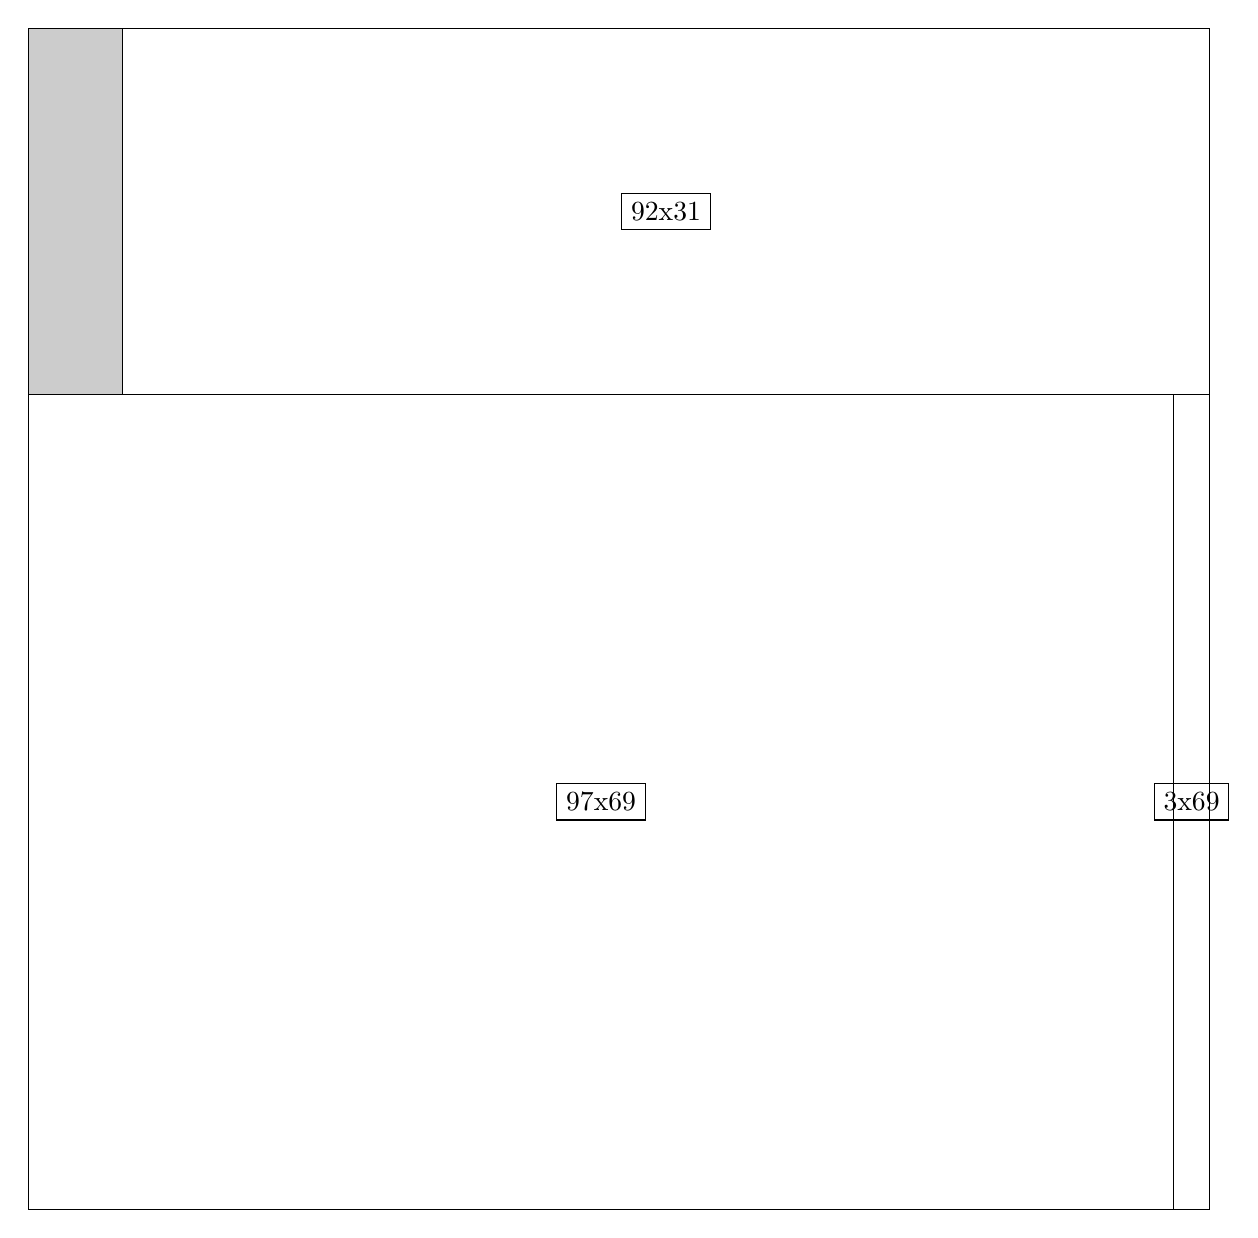
\begin{tikzpicture}[shorten >=1pt,scale=1.0,every node/.style={scale=1.0},->]
\tikzstyle{vertex}=[circle,fill=black!25,minimum size=14pt,inner sep=0pt]
\filldraw[fill=gray!40!white, draw=black] (0,0) rectangle (15.0,15.0);
\foreach \name/\x/\y/\w/\h in {97x69/0.0/0.0/14.549999999999999/10.35,92x31/1.2/10.35/13.799999999999999/4.6499999999999995,3x69/14.549999999999999/0.0/0.44999999999999996/10.35}
\filldraw[fill=white!40!white, draw=black] (\x,\y) rectangle node[draw] (\name) {\name} ++(\w,\h);
\end{tikzpicture}


w =97 , h =69 , x =0 , y =0 , v =6693
\par
w =92 , h =31 , x =8 , y =69 , v =2852
\par
w =3 , h =69 , x =97 , y =0 , v =207
\par
\newpage


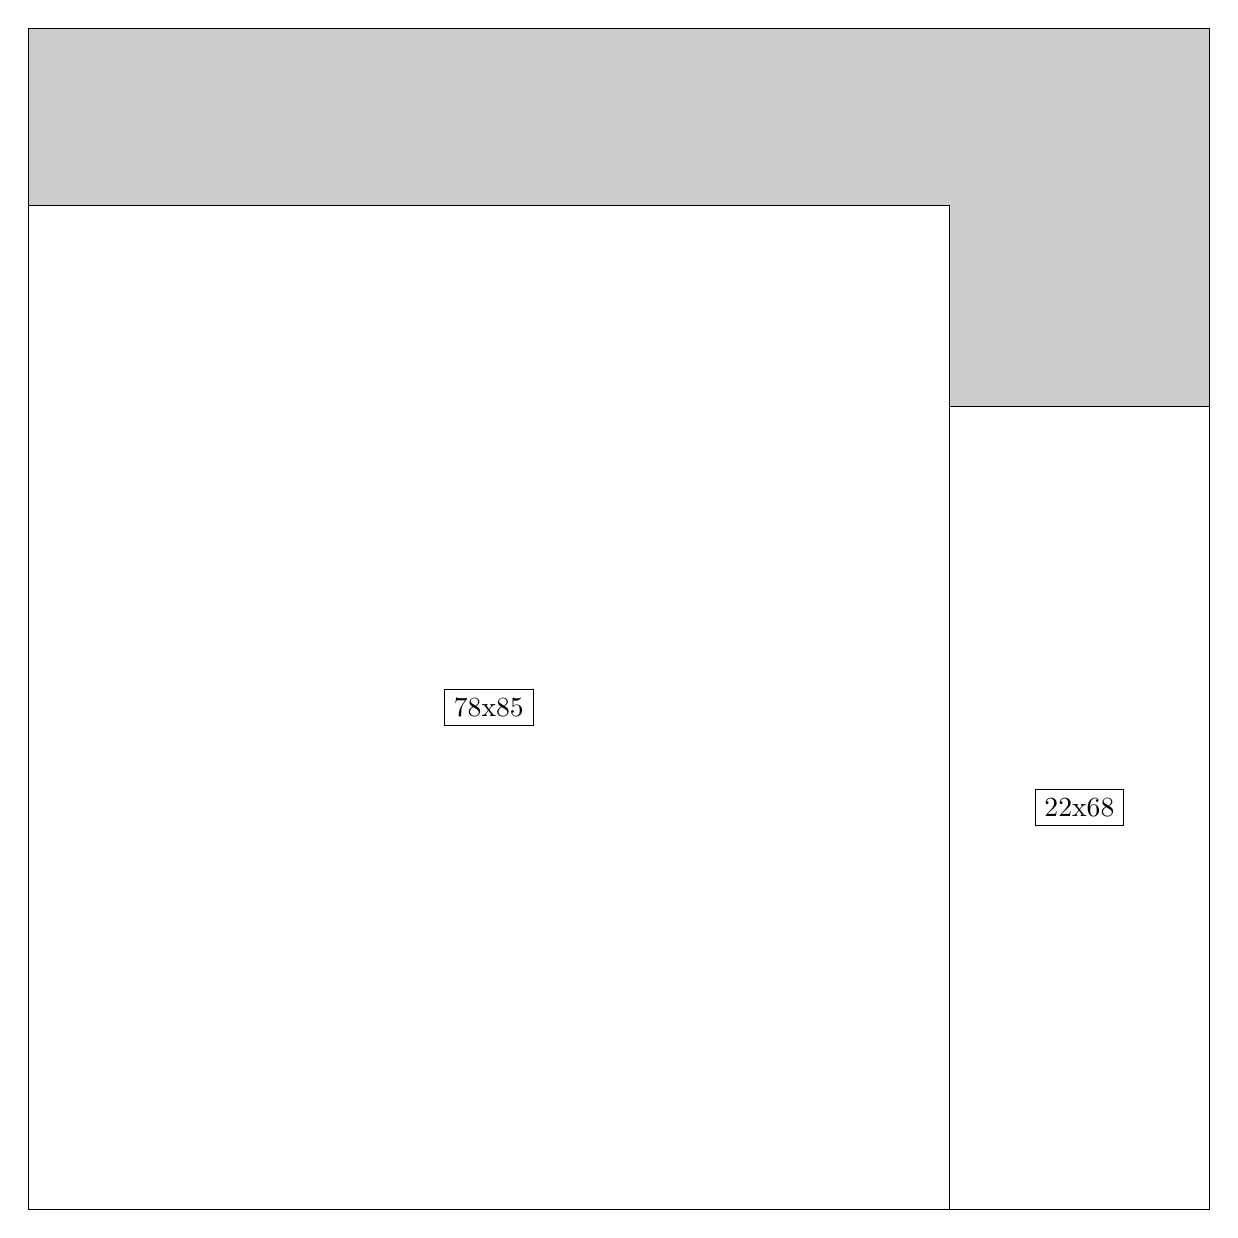
\begin{tikzpicture}[shorten >=1pt,scale=1.0,every node/.style={scale=1.0},->]
\tikzstyle{vertex}=[circle,fill=black!25,minimum size=14pt,inner sep=0pt]
\filldraw[fill=gray!40!white, draw=black] (0,0) rectangle (15.0,15.0);
\foreach \name/\x/\y/\w/\h in {78x85/0.0/0.0/11.7/12.75,22x68/11.7/0.0/3.3/10.2}
\filldraw[fill=white!40!white, draw=black] (\x,\y) rectangle node[draw] (\name) {\name} ++(\w,\h);
\end{tikzpicture}


w =78 , h =85 , x =0 , y =0 , v =6630
\par
w =22 , h =68 , x =78 , y =0 , v =1496
\par
\newpage


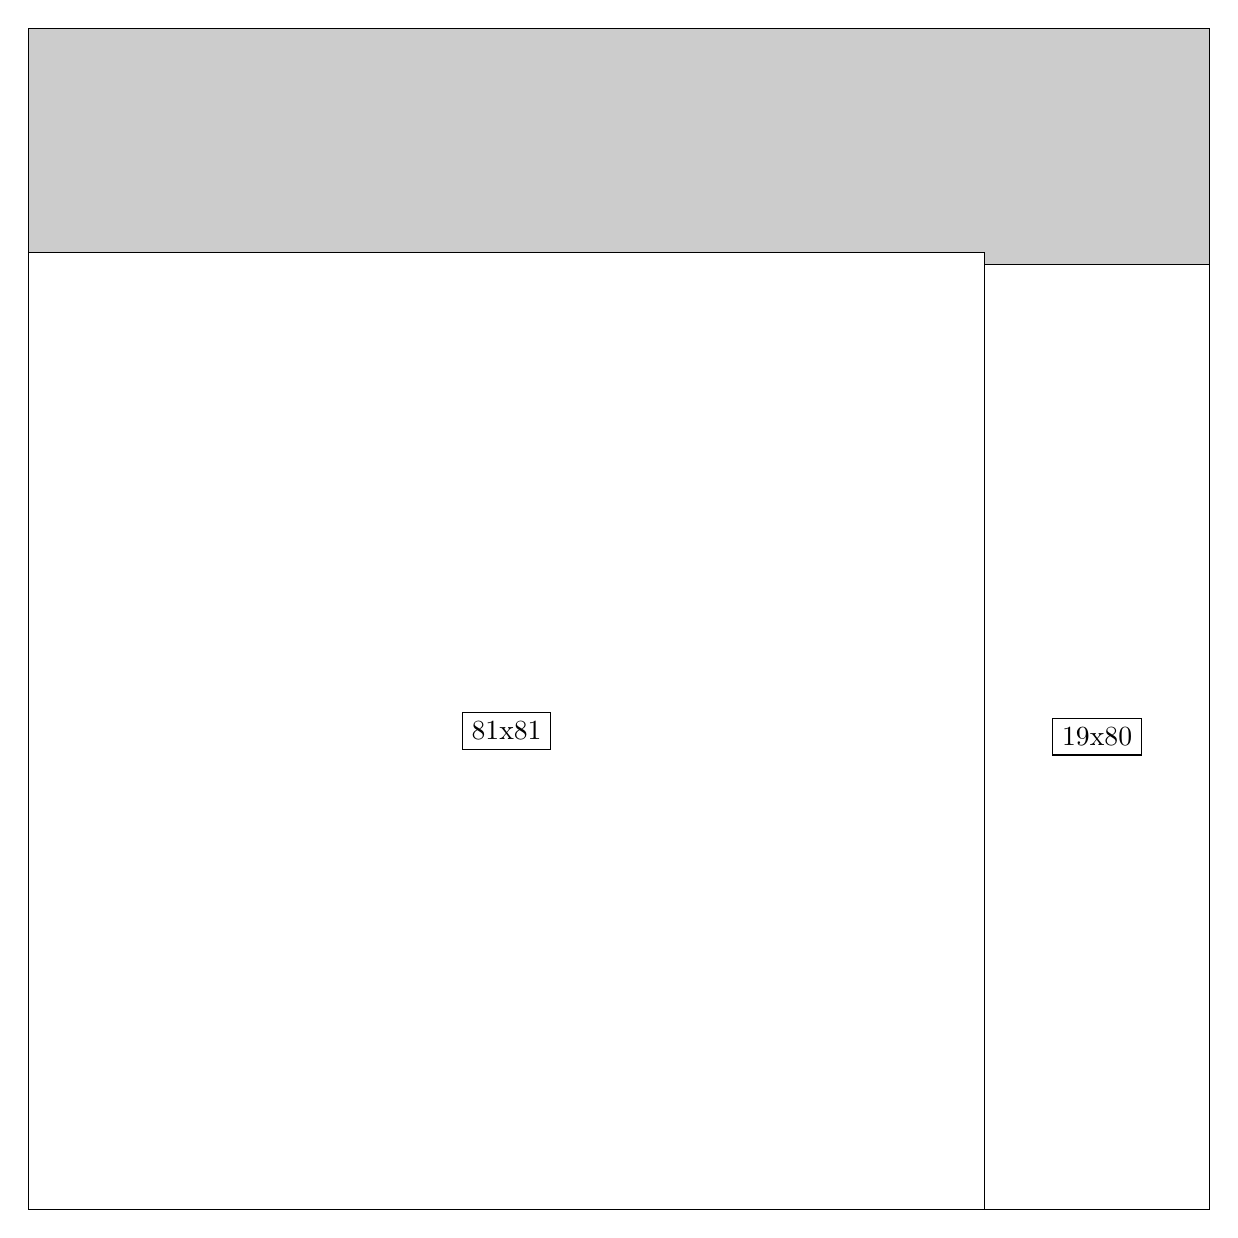
\begin{tikzpicture}[shorten >=1pt,scale=1.0,every node/.style={scale=1.0},->]
\tikzstyle{vertex}=[circle,fill=black!25,minimum size=14pt,inner sep=0pt]
\filldraw[fill=gray!40!white, draw=black] (0,0) rectangle (15.0,15.0);
\foreach \name/\x/\y/\w/\h in {81x81/0.0/0.0/12.15/12.15,19x80/12.15/0.0/2.85/12.0}
\filldraw[fill=white!40!white, draw=black] (\x,\y) rectangle node[draw] (\name) {\name} ++(\w,\h);
\end{tikzpicture}


w =81 , h =81 , x =0 , y =0 , v =6561
\par
w =19 , h =80 , x =81 , y =0 , v =1520
\par
\newpage


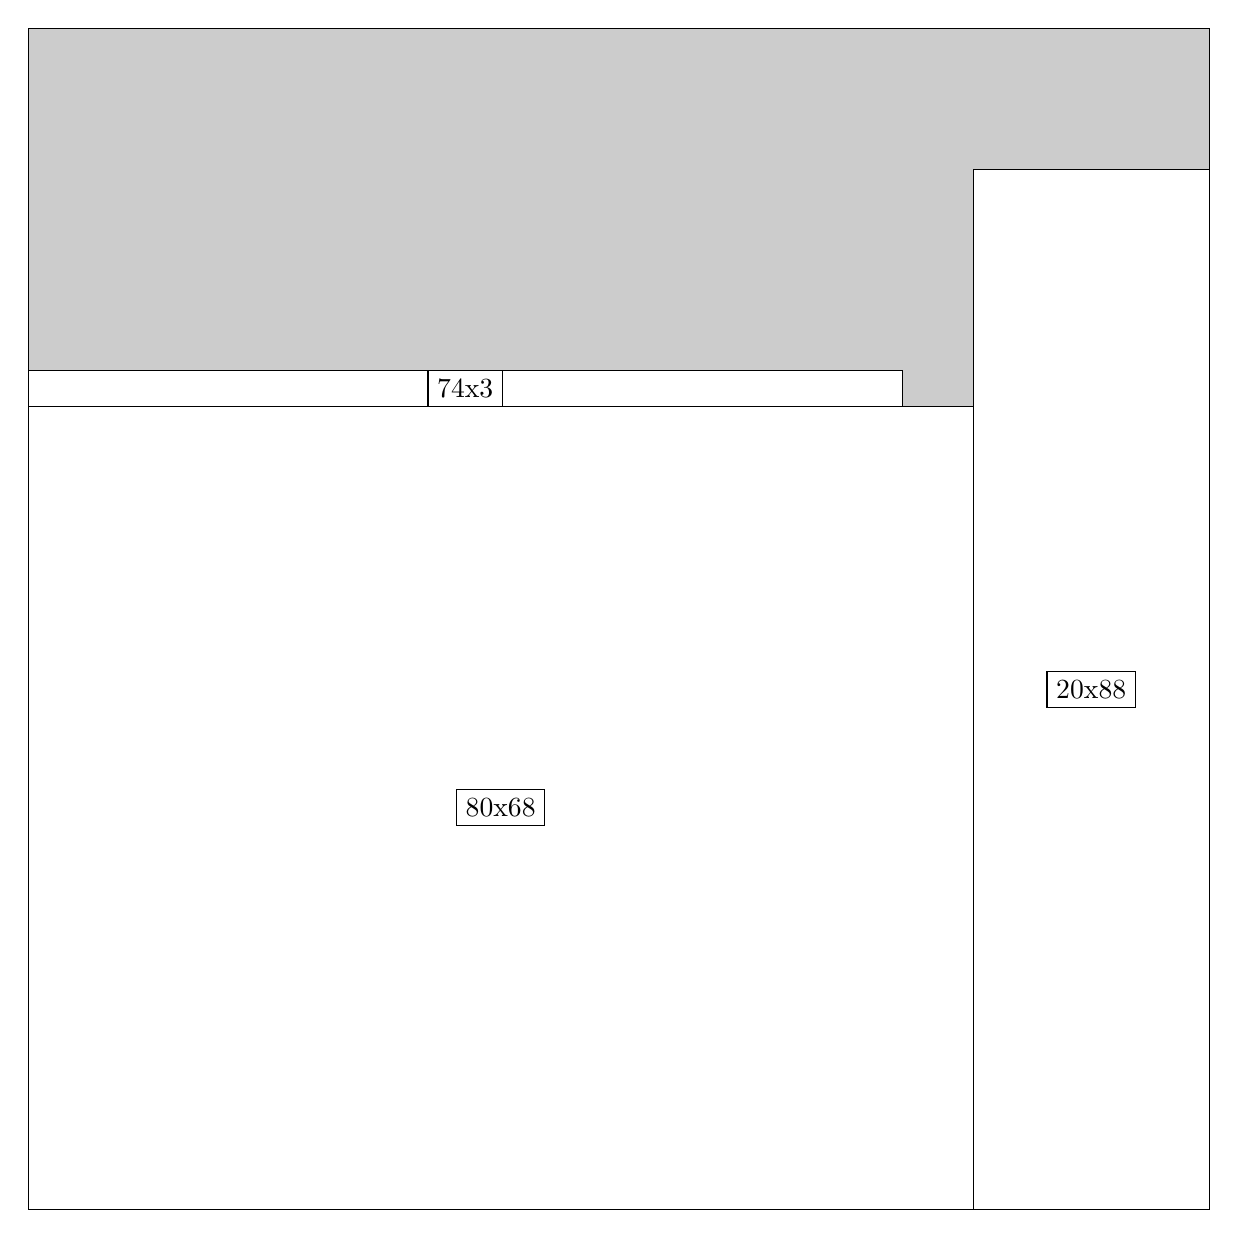
\begin{tikzpicture}[shorten >=1pt,scale=1.0,every node/.style={scale=1.0},->]
\tikzstyle{vertex}=[circle,fill=black!25,minimum size=14pt,inner sep=0pt]
\filldraw[fill=gray!40!white, draw=black] (0,0) rectangle (15.0,15.0);
\foreach \name/\x/\y/\w/\h in {80x68/0.0/0.0/12.0/10.2,20x88/12.0/0.0/3.0/13.2,74x3/0.0/10.2/11.1/0.44999999999999996}
\filldraw[fill=white!40!white, draw=black] (\x,\y) rectangle node[draw] (\name) {\name} ++(\w,\h);
\end{tikzpicture}


w =80 , h =68 , x =0 , y =0 , v =5440
\par
w =20 , h =88 , x =80 , y =0 , v =1760
\par
w =74 , h =3 , x =0 , y =68 , v =222
\par
\newpage


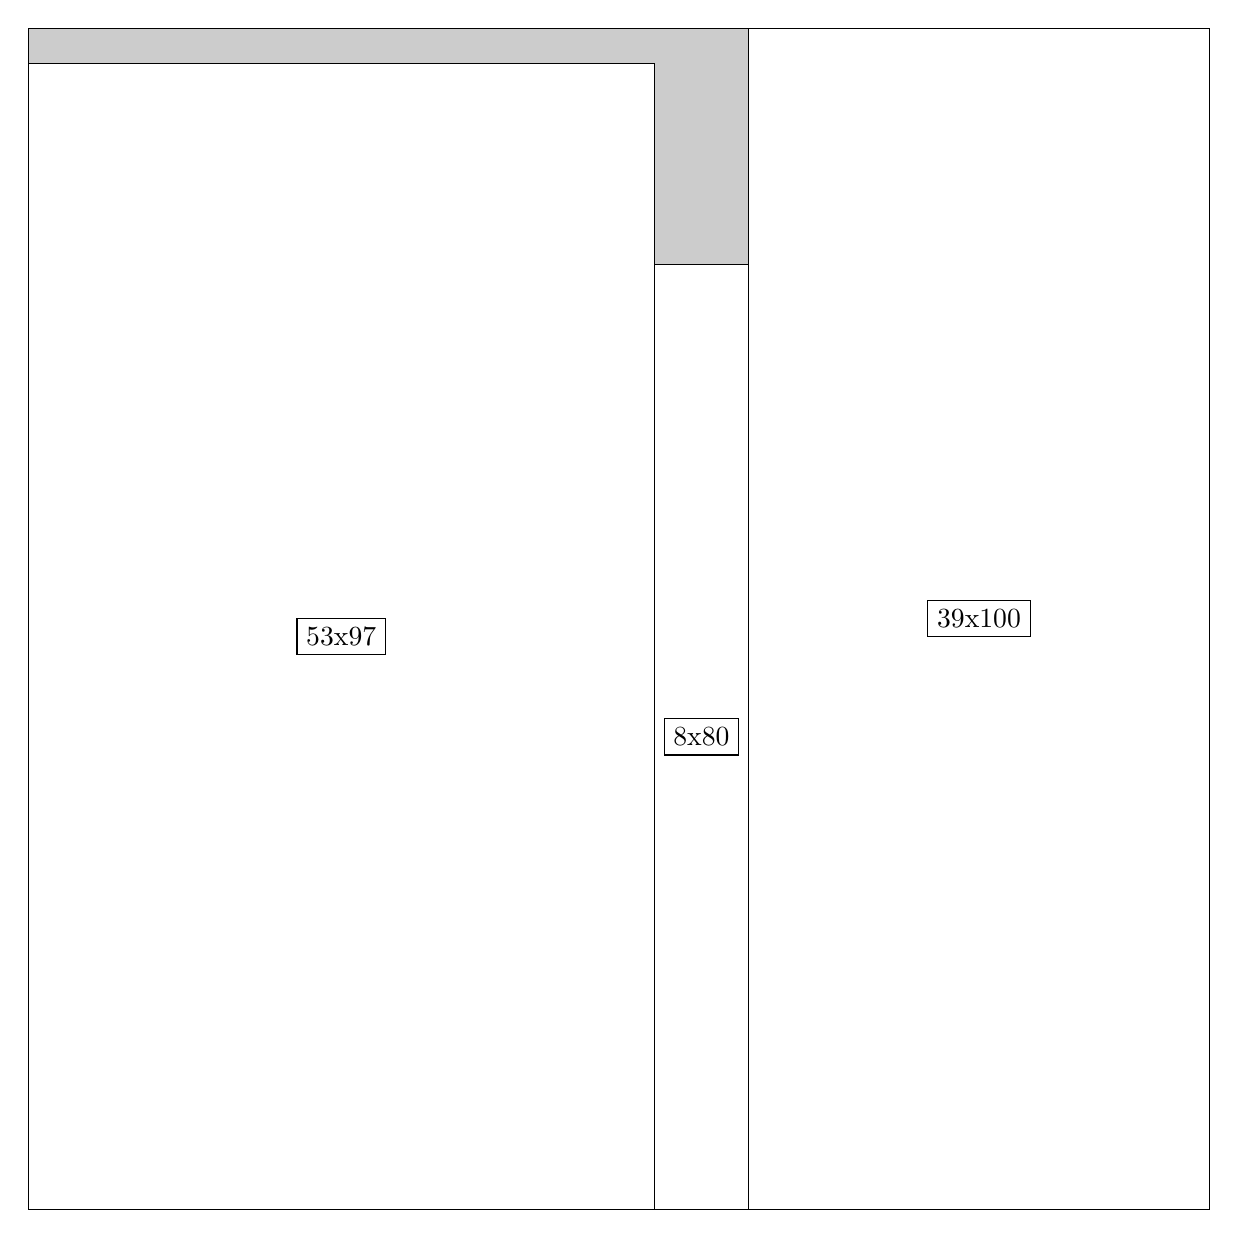
\begin{tikzpicture}[shorten >=1pt,scale=1.0,every node/.style={scale=1.0},->]
\tikzstyle{vertex}=[circle,fill=black!25,minimum size=14pt,inner sep=0pt]
\filldraw[fill=gray!40!white, draw=black] (0,0) rectangle (15.0,15.0);
\foreach \name/\x/\y/\w/\h in {53x97/0.0/0.0/7.949999999999999/14.549999999999999,39x100/9.15/0.0/5.85/15.0,8x80/7.949999999999999/0.0/1.2/12.0}
\filldraw[fill=white!40!white, draw=black] (\x,\y) rectangle node[draw] (\name) {\name} ++(\w,\h);
\end{tikzpicture}


w =53 , h =97 , x =0 , y =0 , v =5141
\par
w =39 , h =100 , x =61 , y =0 , v =3900
\par
w =8 , h =80 , x =53 , y =0 , v =640
\par
\newpage


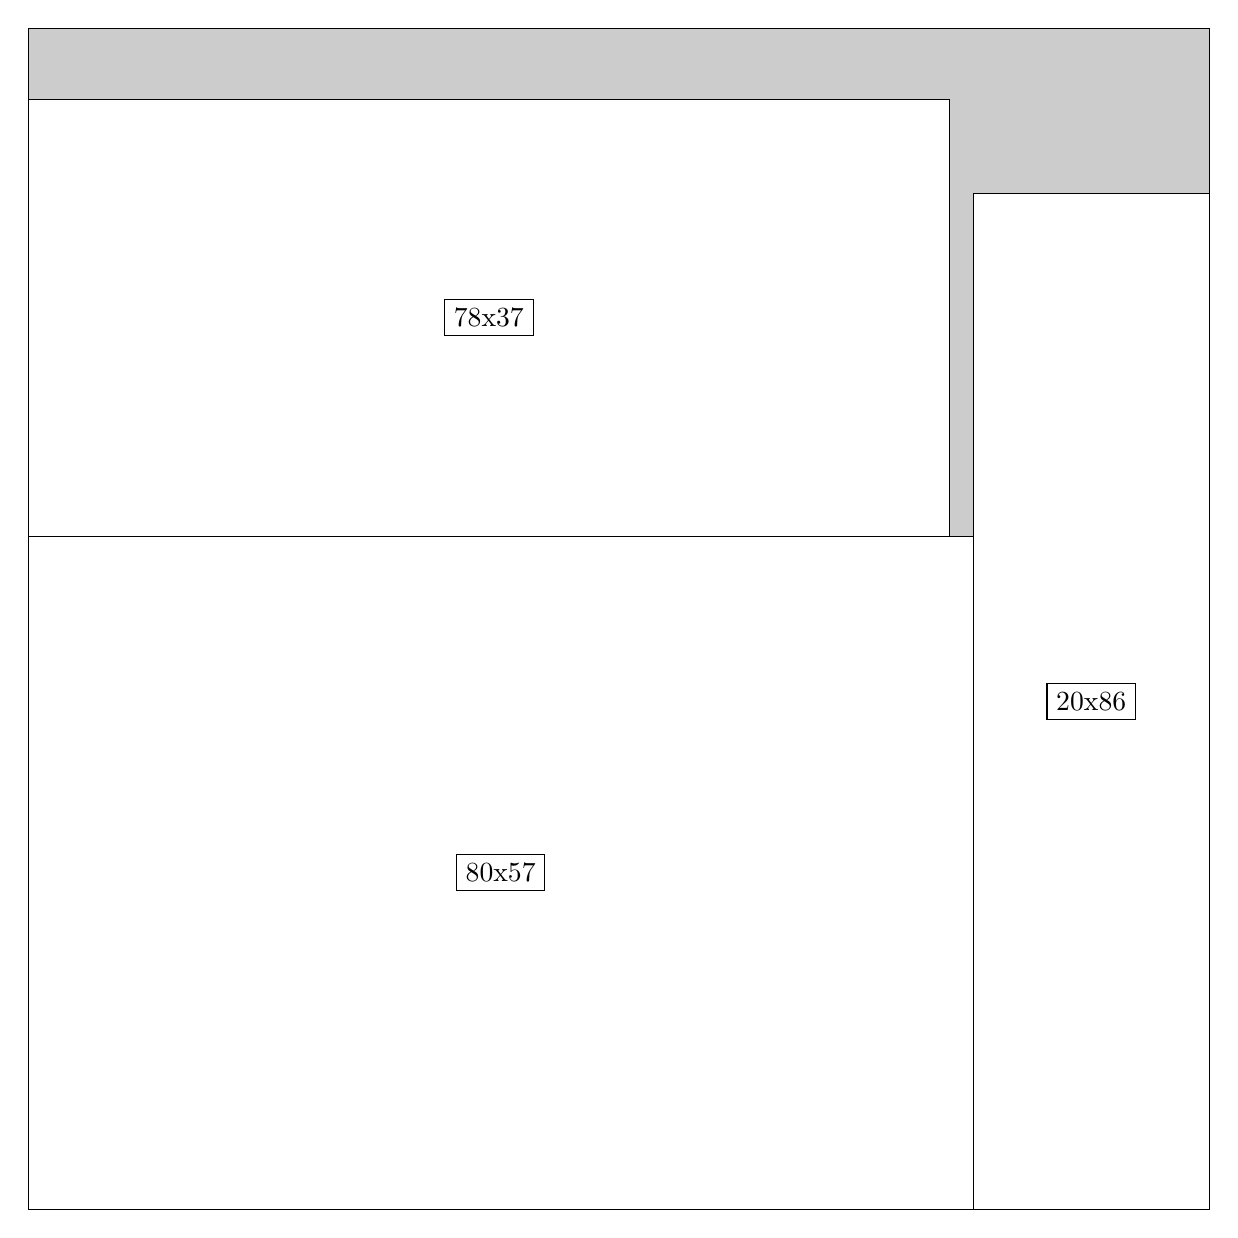
\begin{tikzpicture}[shorten >=1pt,scale=1.0,every node/.style={scale=1.0},->]
\tikzstyle{vertex}=[circle,fill=black!25,minimum size=14pt,inner sep=0pt]
\filldraw[fill=gray!40!white, draw=black] (0,0) rectangle (15.0,15.0);
\foreach \name/\x/\y/\w/\h in {80x57/0.0/0.0/12.0/8.549999999999999,78x37/0.0/8.549999999999999/11.7/5.55,20x86/12.0/0.0/3.0/12.9}
\filldraw[fill=white!40!white, draw=black] (\x,\y) rectangle node[draw] (\name) {\name} ++(\w,\h);
\end{tikzpicture}


w =80 , h =57 , x =0 , y =0 , v =4560
\par
w =78 , h =37 , x =0 , y =57 , v =2886
\par
w =20 , h =86 , x =80 , y =0 , v =1720
\par
\newpage


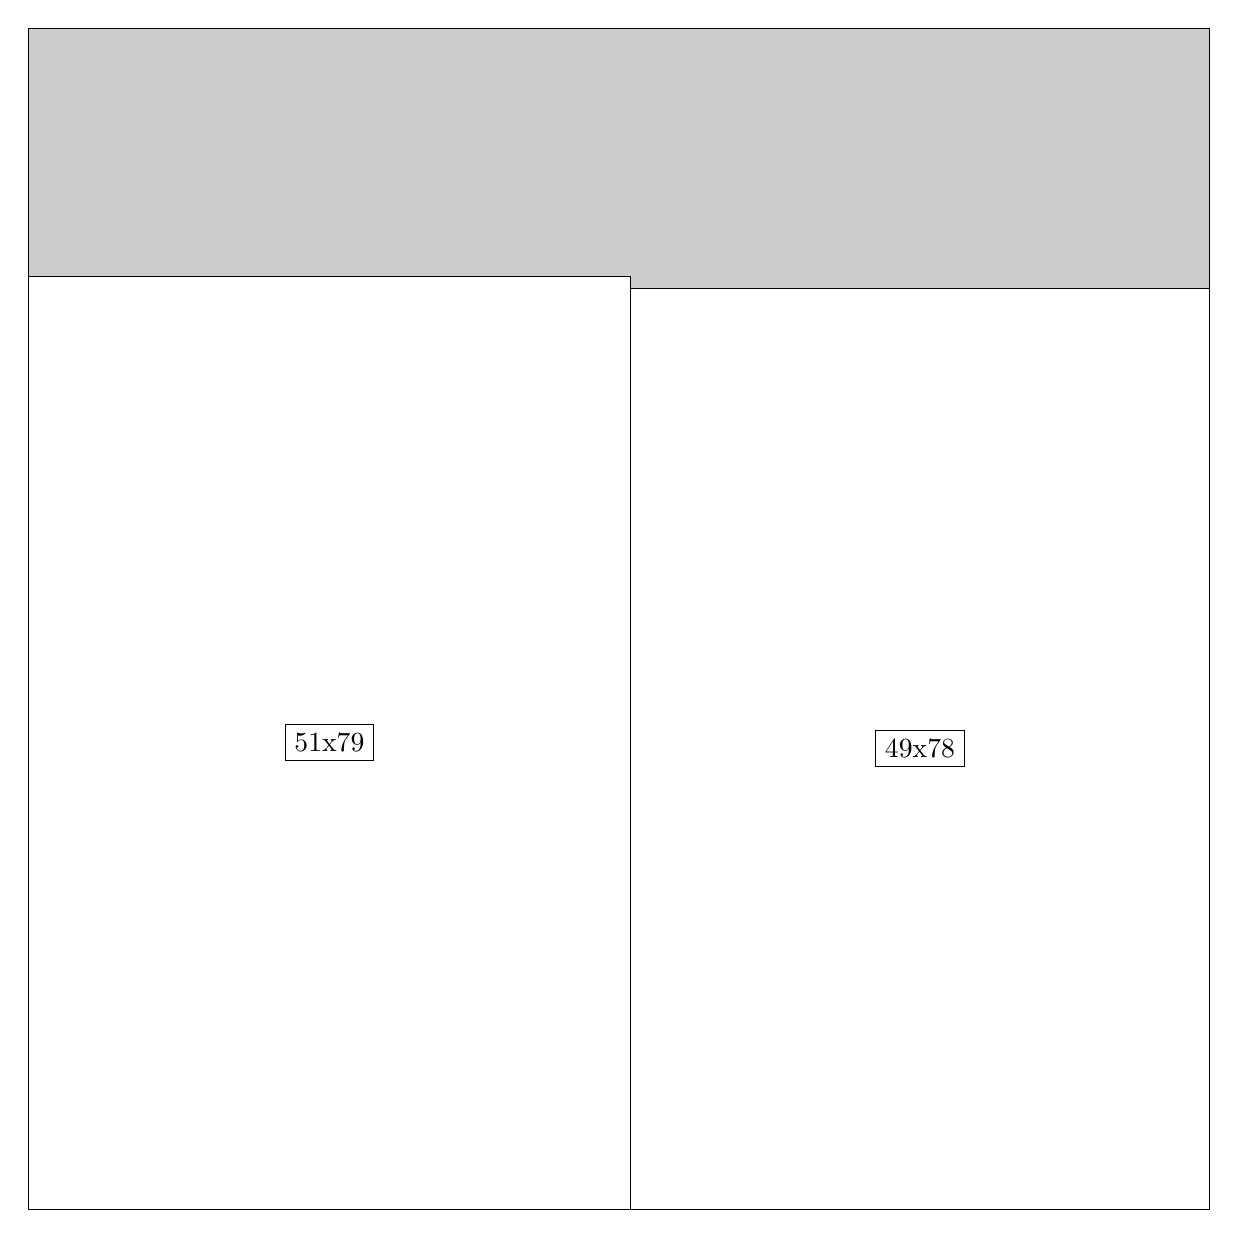
\begin{tikzpicture}[shorten >=1pt,scale=1.0,every node/.style={scale=1.0},->]
\tikzstyle{vertex}=[circle,fill=black!25,minimum size=14pt,inner sep=0pt]
\filldraw[fill=gray!40!white, draw=black] (0,0) rectangle (15.0,15.0);
\foreach \name/\x/\y/\w/\h in {51x79/0.0/0.0/7.6499999999999995/11.85,49x78/7.6499999999999995/0.0/7.35/11.7}
\filldraw[fill=white!40!white, draw=black] (\x,\y) rectangle node[draw] (\name) {\name} ++(\w,\h);
\end{tikzpicture}


w =51 , h =79 , x =0 , y =0 , v =4029
\par
w =49 , h =78 , x =51 , y =0 , v =3822
\par
\newpage


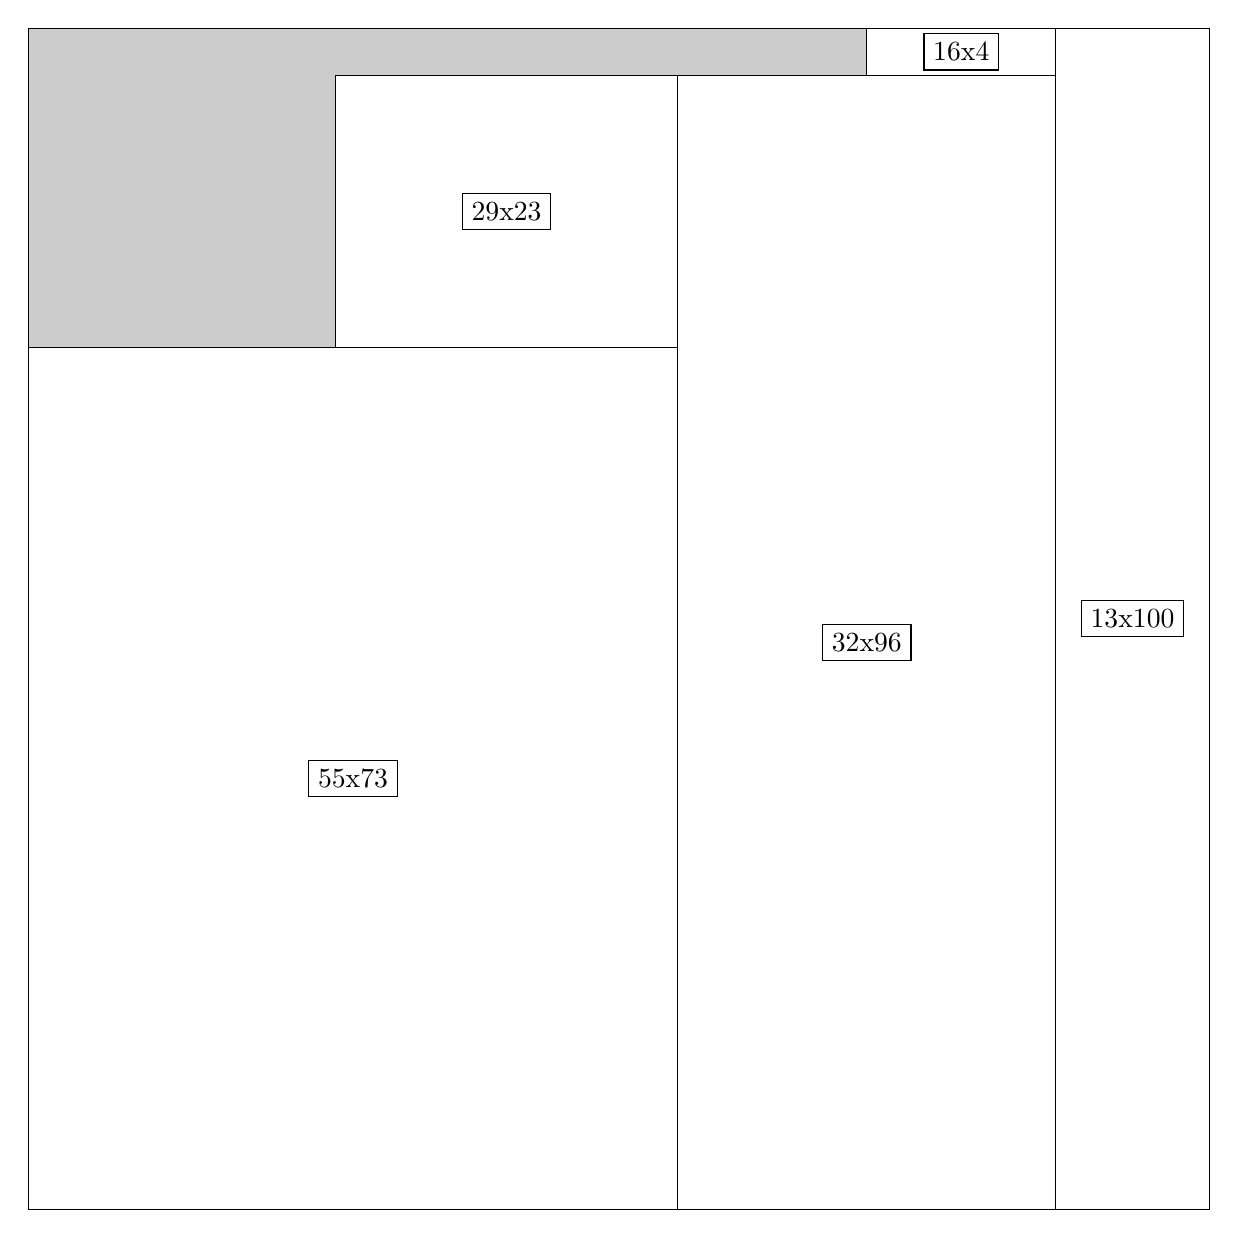
\begin{tikzpicture}[shorten >=1pt,scale=1.0,every node/.style={scale=1.0},->]
\tikzstyle{vertex}=[circle,fill=black!25,minimum size=14pt,inner sep=0pt]
\filldraw[fill=gray!40!white, draw=black] (0,0) rectangle (15.0,15.0);
\foreach \name/\x/\y/\w/\h in {55x73/0.0/0.0/8.25/10.95,32x96/8.25/0.0/4.8/14.399999999999999,13x100/13.049999999999999/0.0/1.95/15.0,29x23/3.9/10.95/4.35/3.4499999999999997,16x4/10.65/14.399999999999999/2.4/0.6}
\filldraw[fill=white!40!white, draw=black] (\x,\y) rectangle node[draw] (\name) {\name} ++(\w,\h);
\end{tikzpicture}


w =55 , h =73 , x =0 , y =0 , v =4015
\par
w =32 , h =96 , x =55 , y =0 , v =3072
\par
w =13 , h =100 , x =87 , y =0 , v =1300
\par
w =29 , h =23 , x =26 , y =73 , v =667
\par
w =16 , h =4 , x =71 , y =96 , v =64
\par
\newpage


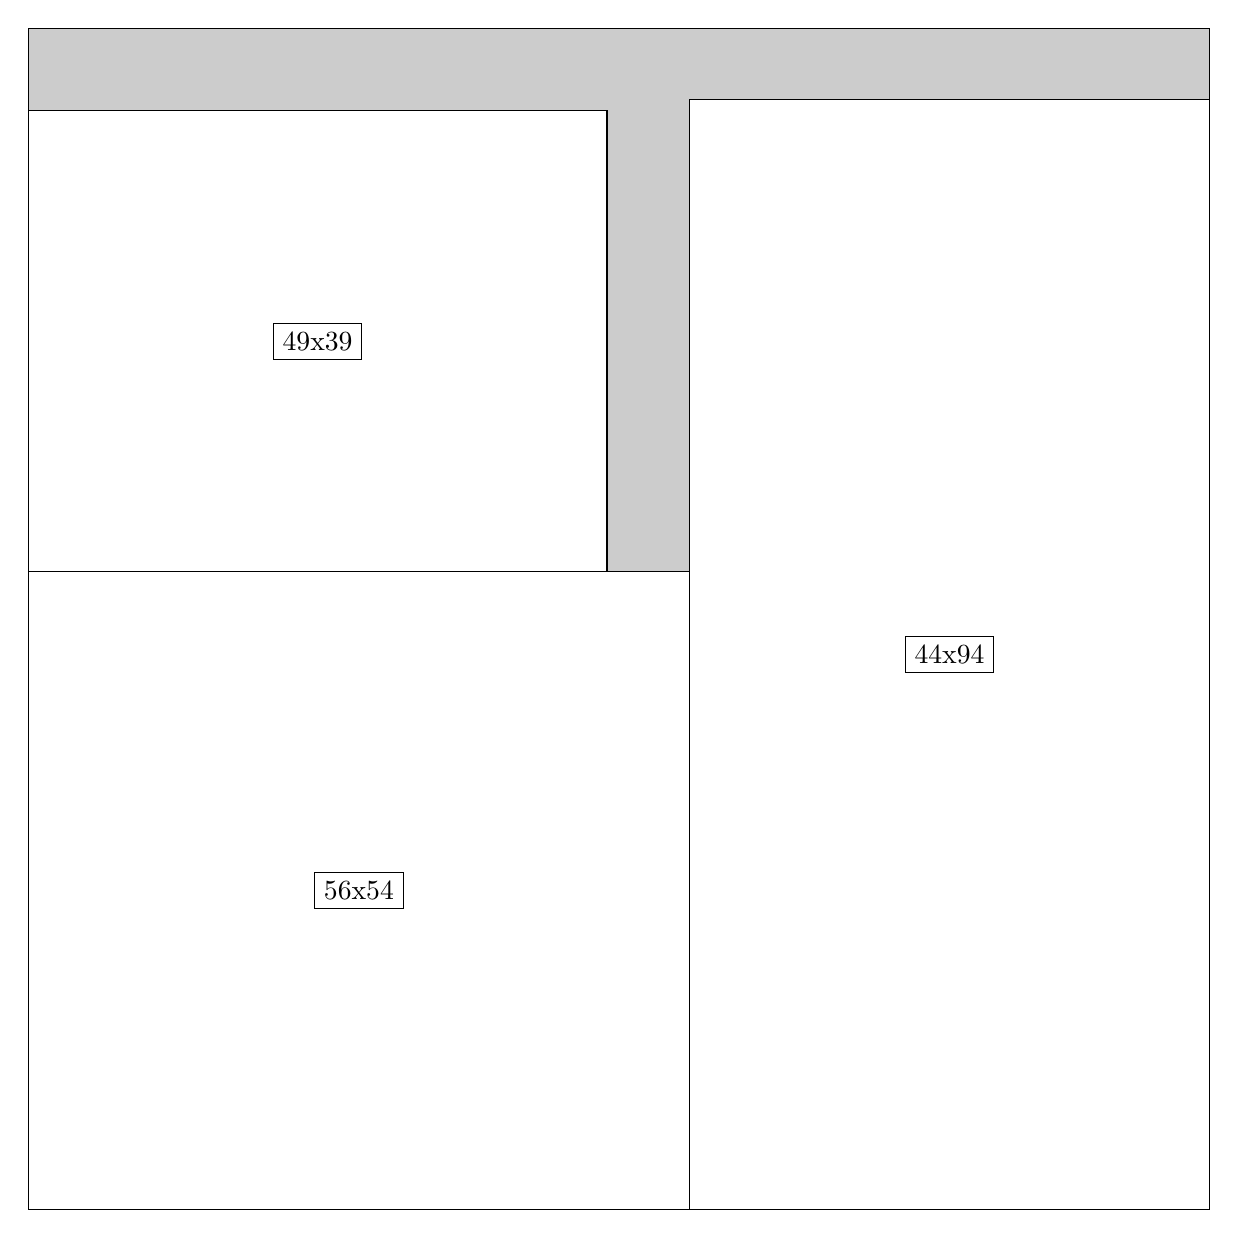
\begin{tikzpicture}[shorten >=1pt,scale=1.0,every node/.style={scale=1.0},->]
\tikzstyle{vertex}=[circle,fill=black!25,minimum size=14pt,inner sep=0pt]
\filldraw[fill=gray!40!white, draw=black] (0,0) rectangle (15.0,15.0);
\foreach \name/\x/\y/\w/\h in {44x94/8.4/0.0/6.6/14.1,56x54/0.0/0.0/8.4/8.1,49x39/0.0/8.1/7.35/5.85}
\filldraw[fill=white!40!white, draw=black] (\x,\y) rectangle node[draw] (\name) {\name} ++(\w,\h);
\end{tikzpicture}


w =44 , h =94 , x =56 , y =0 , v =4136
\par
w =56 , h =54 , x =0 , y =0 , v =3024
\par
w =49 , h =39 , x =0 , y =54 , v =1911
\par
\newpage


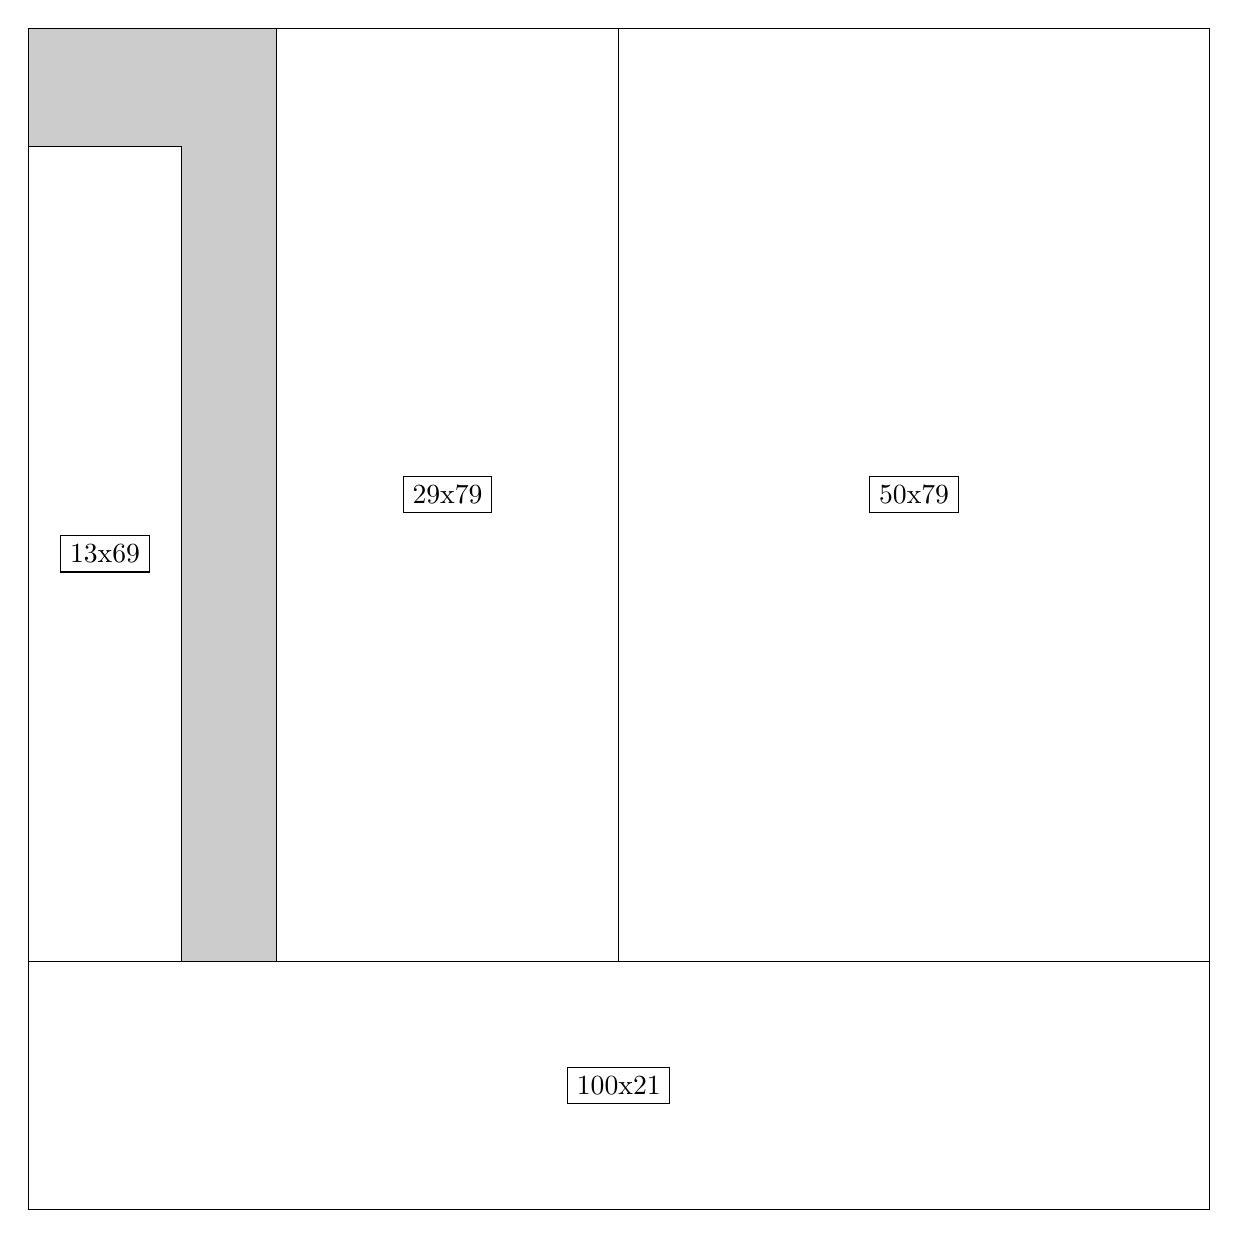
\begin{tikzpicture}[shorten >=1pt,scale=1.0,every node/.style={scale=1.0},->]
\tikzstyle{vertex}=[circle,fill=black!25,minimum size=14pt,inner sep=0pt]
\filldraw[fill=gray!40!white, draw=black] (0,0) rectangle (15.0,15.0);
\foreach \name/\x/\y/\w/\h in {50x79/7.5/3.15/7.5/11.85,29x79/3.15/3.15/4.35/11.85,100x21/0.0/0.0/15.0/3.15,13x69/0.0/3.15/1.95/10.35}
\filldraw[fill=white!40!white, draw=black] (\x,\y) rectangle node[draw] (\name) {\name} ++(\w,\h);
\end{tikzpicture}


w =50 , h =79 , x =50 , y =21 , v =3950
\par
w =29 , h =79 , x =21 , y =21 , v =2291
\par
w =100 , h =21 , x =0 , y =0 , v =2100
\par
w =13 , h =69 , x =0 , y =21 , v =897
\par
\newpage


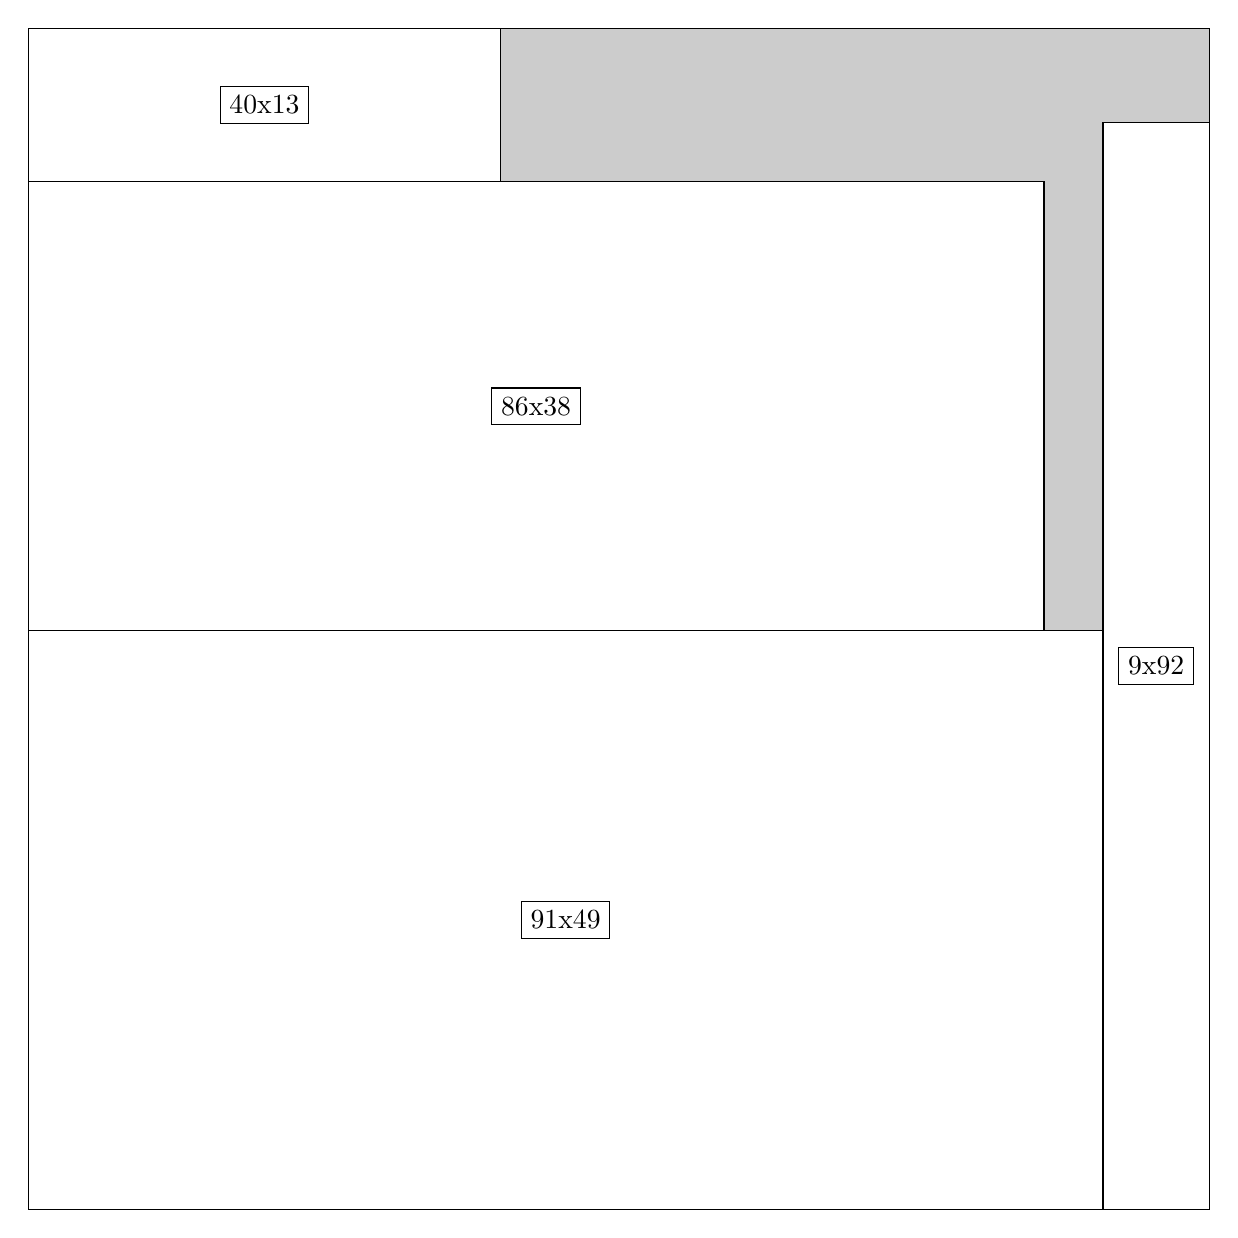
\begin{tikzpicture}[shorten >=1pt,scale=1.0,every node/.style={scale=1.0},->]
\tikzstyle{vertex}=[circle,fill=black!25,minimum size=14pt,inner sep=0pt]
\filldraw[fill=gray!40!white, draw=black] (0,0) rectangle (15.0,15.0);
\foreach \name/\x/\y/\w/\h in {91x49/0.0/0.0/13.65/7.35,86x38/0.0/7.35/12.9/5.7,9x92/13.65/0.0/1.3499999999999999/13.799999999999999,40x13/0.0/13.049999999999999/6.0/1.95}
\filldraw[fill=white!40!white, draw=black] (\x,\y) rectangle node[draw] (\name) {\name} ++(\w,\h);
\end{tikzpicture}


w =91 , h =49 , x =0 , y =0 , v =4459
\par
w =86 , h =38 , x =0 , y =49 , v =3268
\par
w =9 , h =92 , x =91 , y =0 , v =828
\par
w =40 , h =13 , x =0 , y =87 , v =520
\par
\newpage


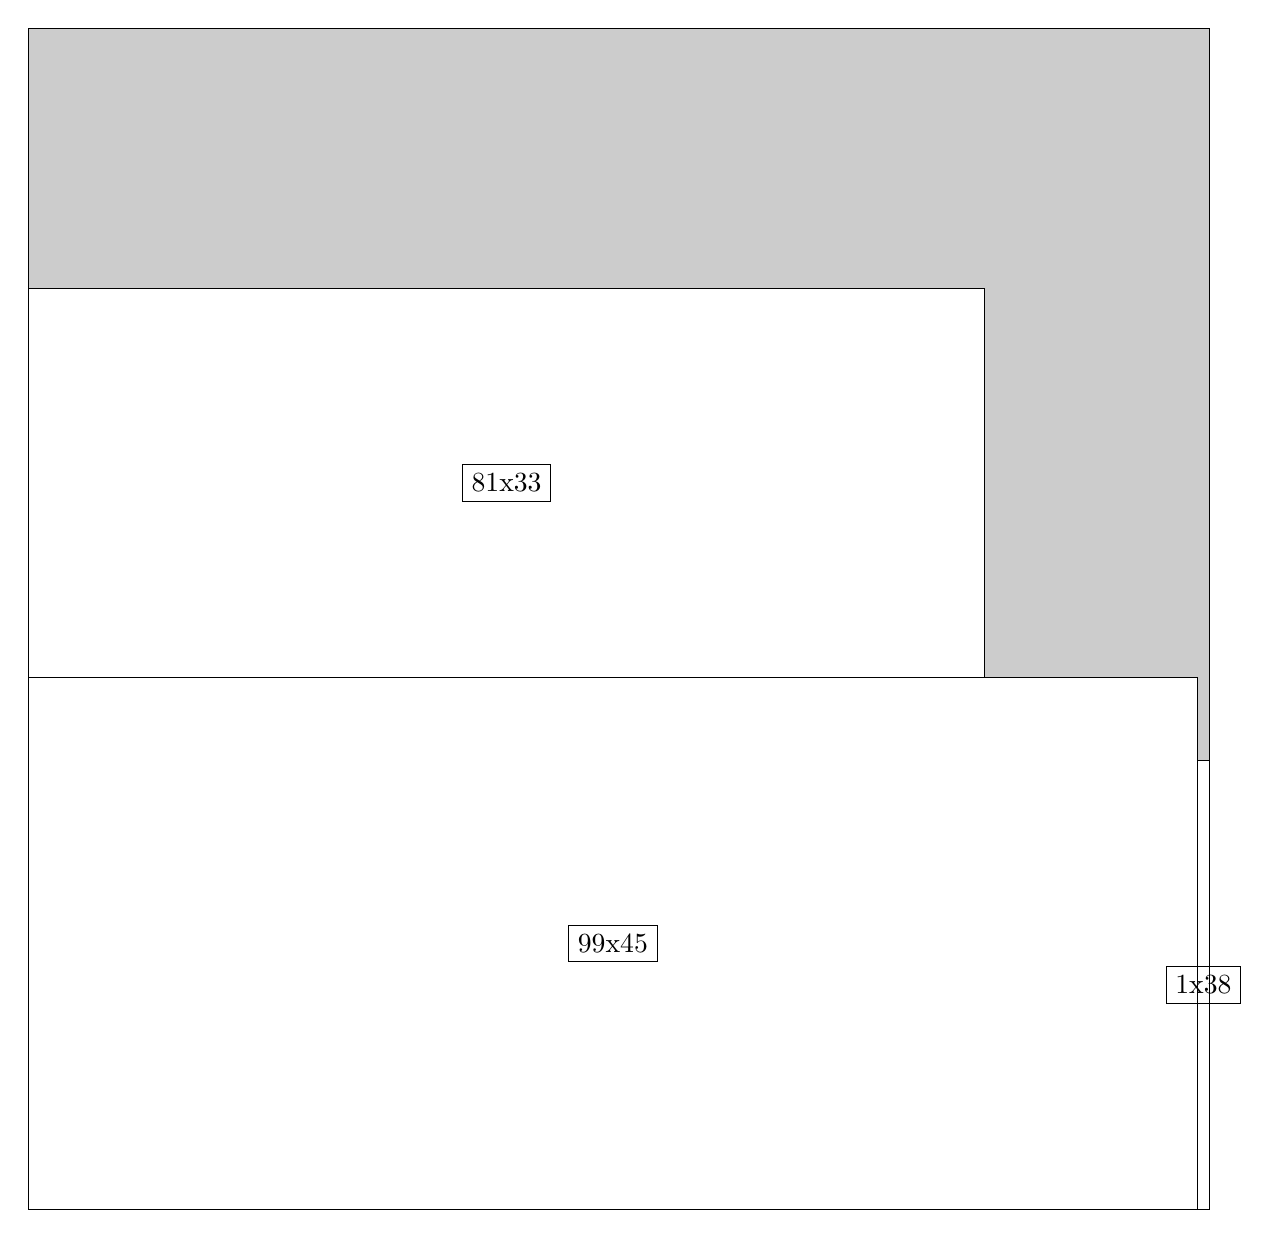
\begin{tikzpicture}[shorten >=1pt,scale=1.0,every node/.style={scale=1.0},->]
\tikzstyle{vertex}=[circle,fill=black!25,minimum size=14pt,inner sep=0pt]
\filldraw[fill=gray!40!white, draw=black] (0,0) rectangle (15.0,15.0);
\foreach \name/\x/\y/\w/\h in {99x45/0.0/0.0/14.85/6.75,81x33/0.0/6.75/12.15/4.95,1x38/14.85/0.0/0.15/5.7}
\filldraw[fill=white!40!white, draw=black] (\x,\y) rectangle node[draw] (\name) {\name} ++(\w,\h);
\end{tikzpicture}


w =99 , h =45 , x =0 , y =0 , v =4455
\par
w =81 , h =33 , x =0 , y =45 , v =2673
\par
w =1 , h =38 , x =99 , y =0 , v =38
\par
\newpage


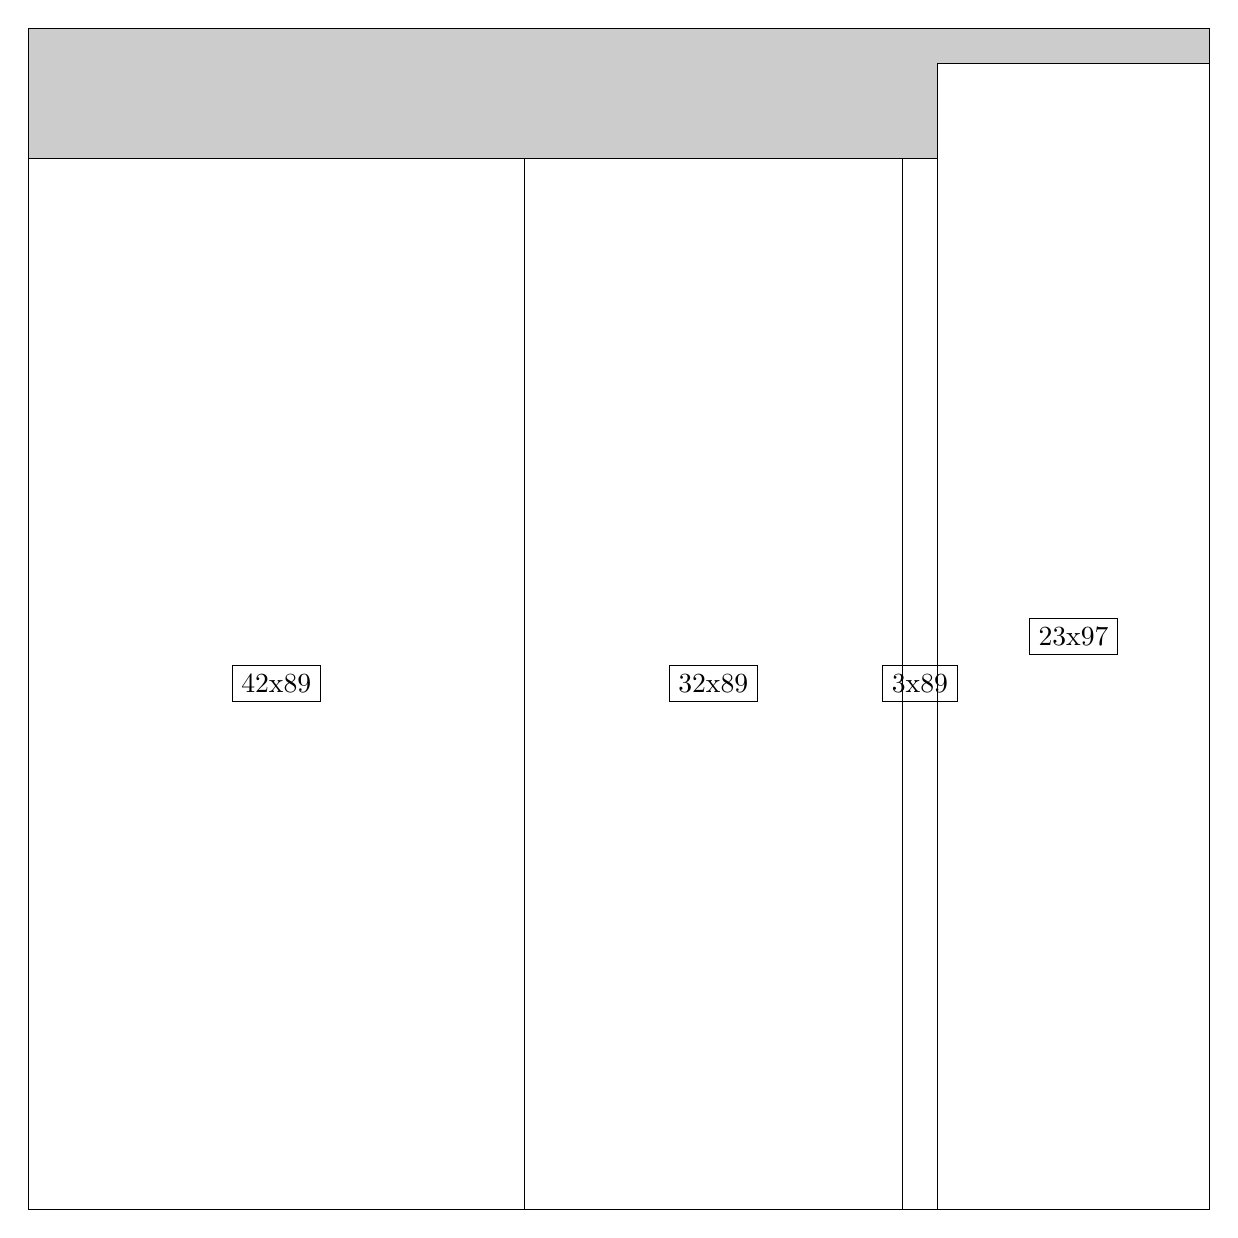
\begin{tikzpicture}[shorten >=1pt,scale=1.0,every node/.style={scale=1.0},->]
\tikzstyle{vertex}=[circle,fill=black!25,minimum size=14pt,inner sep=0pt]
\filldraw[fill=gray!40!white, draw=black] (0,0) rectangle (15.0,15.0);
\foreach \name/\x/\y/\w/\h in {42x89/0.0/0.0/6.3/13.35,32x89/6.3/0.0/4.8/13.35,23x97/11.549999999999999/0.0/3.4499999999999997/14.549999999999999,3x89/11.1/0.0/0.44999999999999996/13.35}
\filldraw[fill=white!40!white, draw=black] (\x,\y) rectangle node[draw] (\name) {\name} ++(\w,\h);
\end{tikzpicture}


w =42 , h =89 , x =0 , y =0 , v =3738
\par
w =32 , h =89 , x =42 , y =0 , v =2848
\par
w =23 , h =97 , x =77 , y =0 , v =2231
\par
w =3 , h =89 , x =74 , y =0 , v =267
\par
\newpage


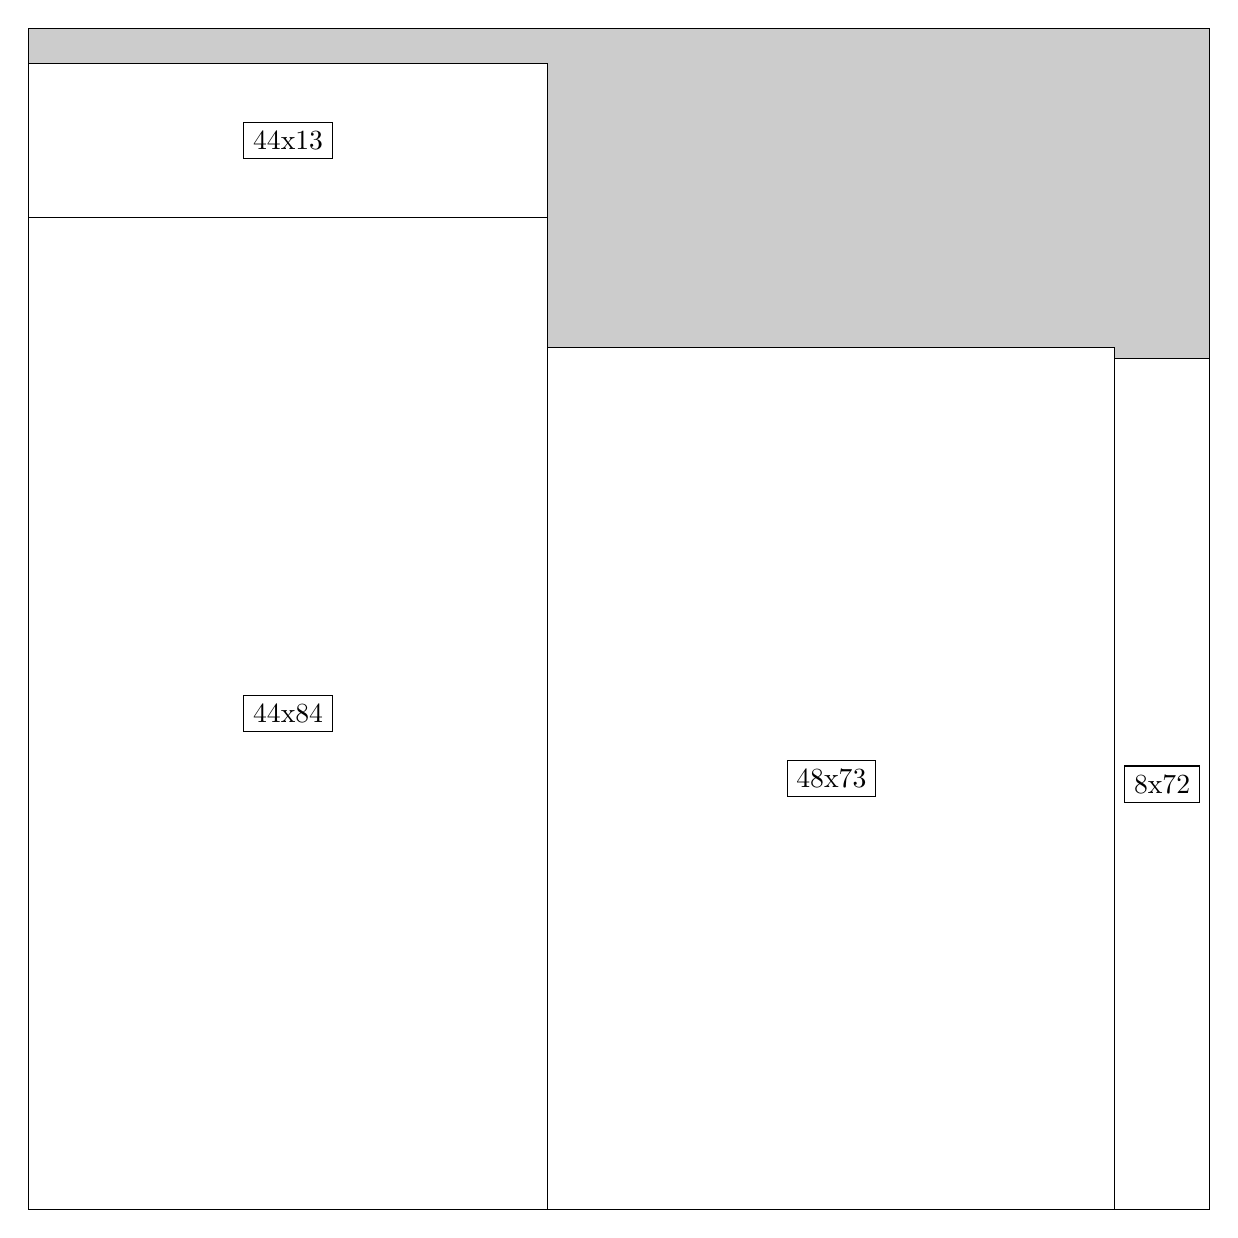
\begin{tikzpicture}[shorten >=1pt,scale=1.0,every node/.style={scale=1.0},->]
\tikzstyle{vertex}=[circle,fill=black!25,minimum size=14pt,inner sep=0pt]
\filldraw[fill=gray!40!white, draw=black] (0,0) rectangle (15.0,15.0);
\foreach \name/\x/\y/\w/\h in {44x84/0.0/0.0/6.6/12.6,48x73/6.6/0.0/7.199999999999999/10.95,8x72/13.799999999999999/0.0/1.2/10.799999999999999,44x13/0.0/12.6/6.6/1.95}
\filldraw[fill=white!40!white, draw=black] (\x,\y) rectangle node[draw] (\name) {\name} ++(\w,\h);
\end{tikzpicture}


w =44 , h =84 , x =0 , y =0 , v =3696
\par
w =48 , h =73 , x =44 , y =0 , v =3504
\par
w =8 , h =72 , x =92 , y =0 , v =576
\par
w =44 , h =13 , x =0 , y =84 , v =572
\par
\newpage


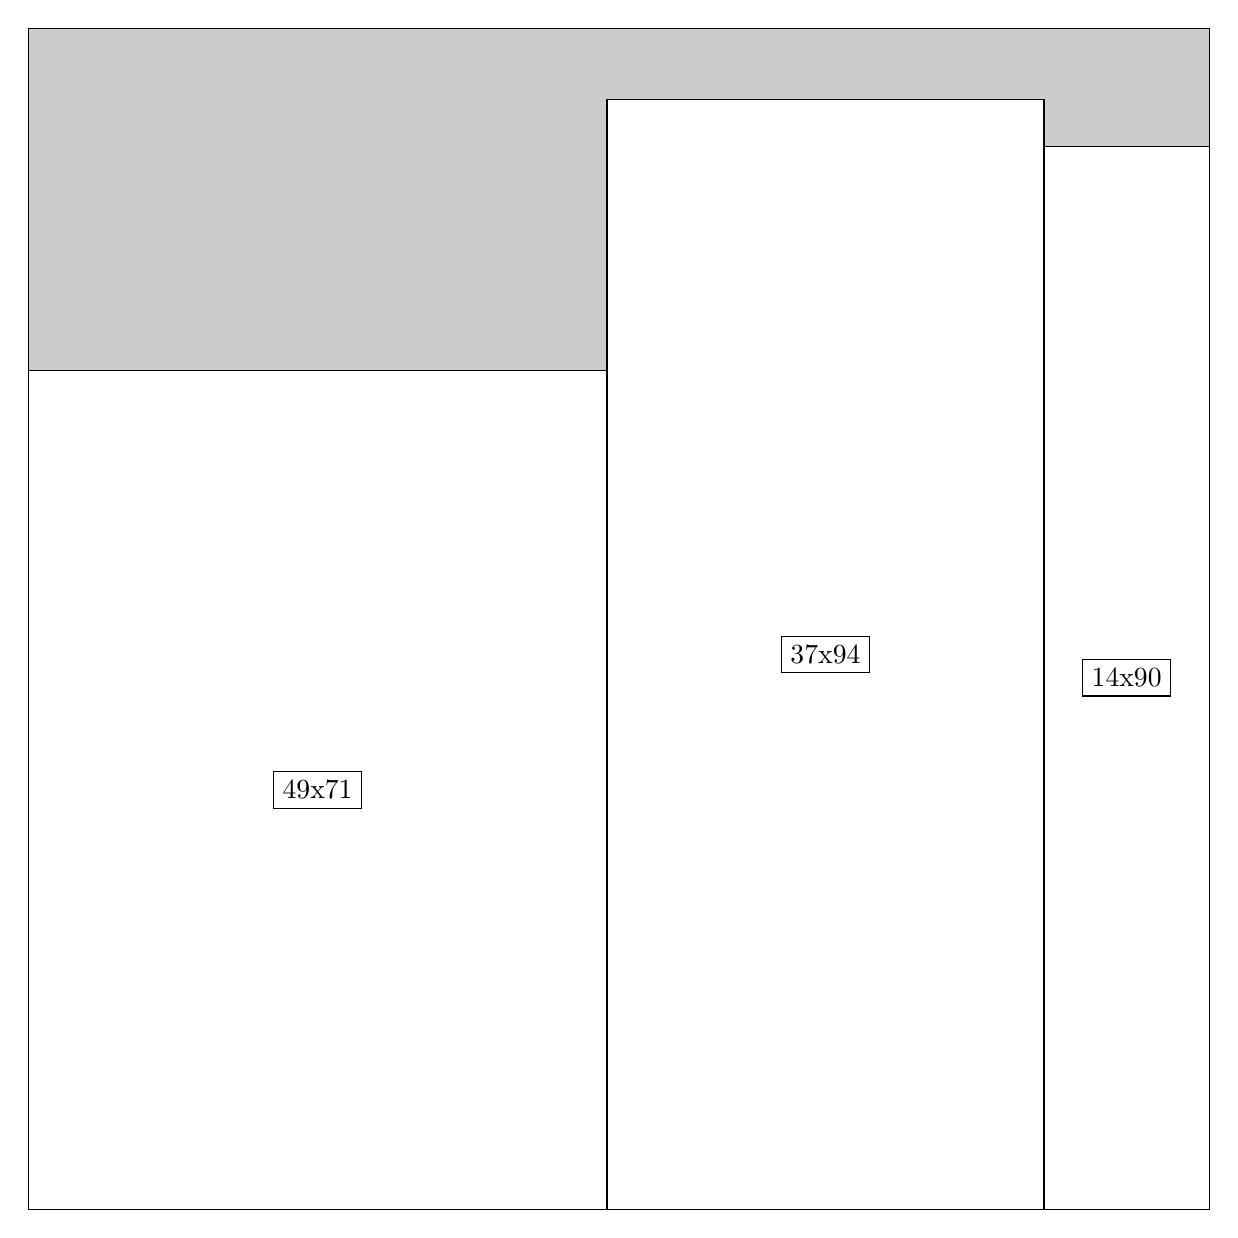
\begin{tikzpicture}[shorten >=1pt,scale=1.0,every node/.style={scale=1.0},->]
\tikzstyle{vertex}=[circle,fill=black!25,minimum size=14pt,inner sep=0pt]
\filldraw[fill=gray!40!white, draw=black] (0,0) rectangle (15.0,15.0);
\foreach \name/\x/\y/\w/\h in {49x71/0.0/0.0/7.35/10.65,37x94/7.35/0.0/5.55/14.1,14x90/12.9/0.0/2.1/13.5}
\filldraw[fill=white!40!white, draw=black] (\x,\y) rectangle node[draw] (\name) {\name} ++(\w,\h);
\end{tikzpicture}


w =49 , h =71 , x =0 , y =0 , v =3479
\par
w =37 , h =94 , x =49 , y =0 , v =3478
\par
w =14 , h =90 , x =86 , y =0 , v =1260
\par
\newpage


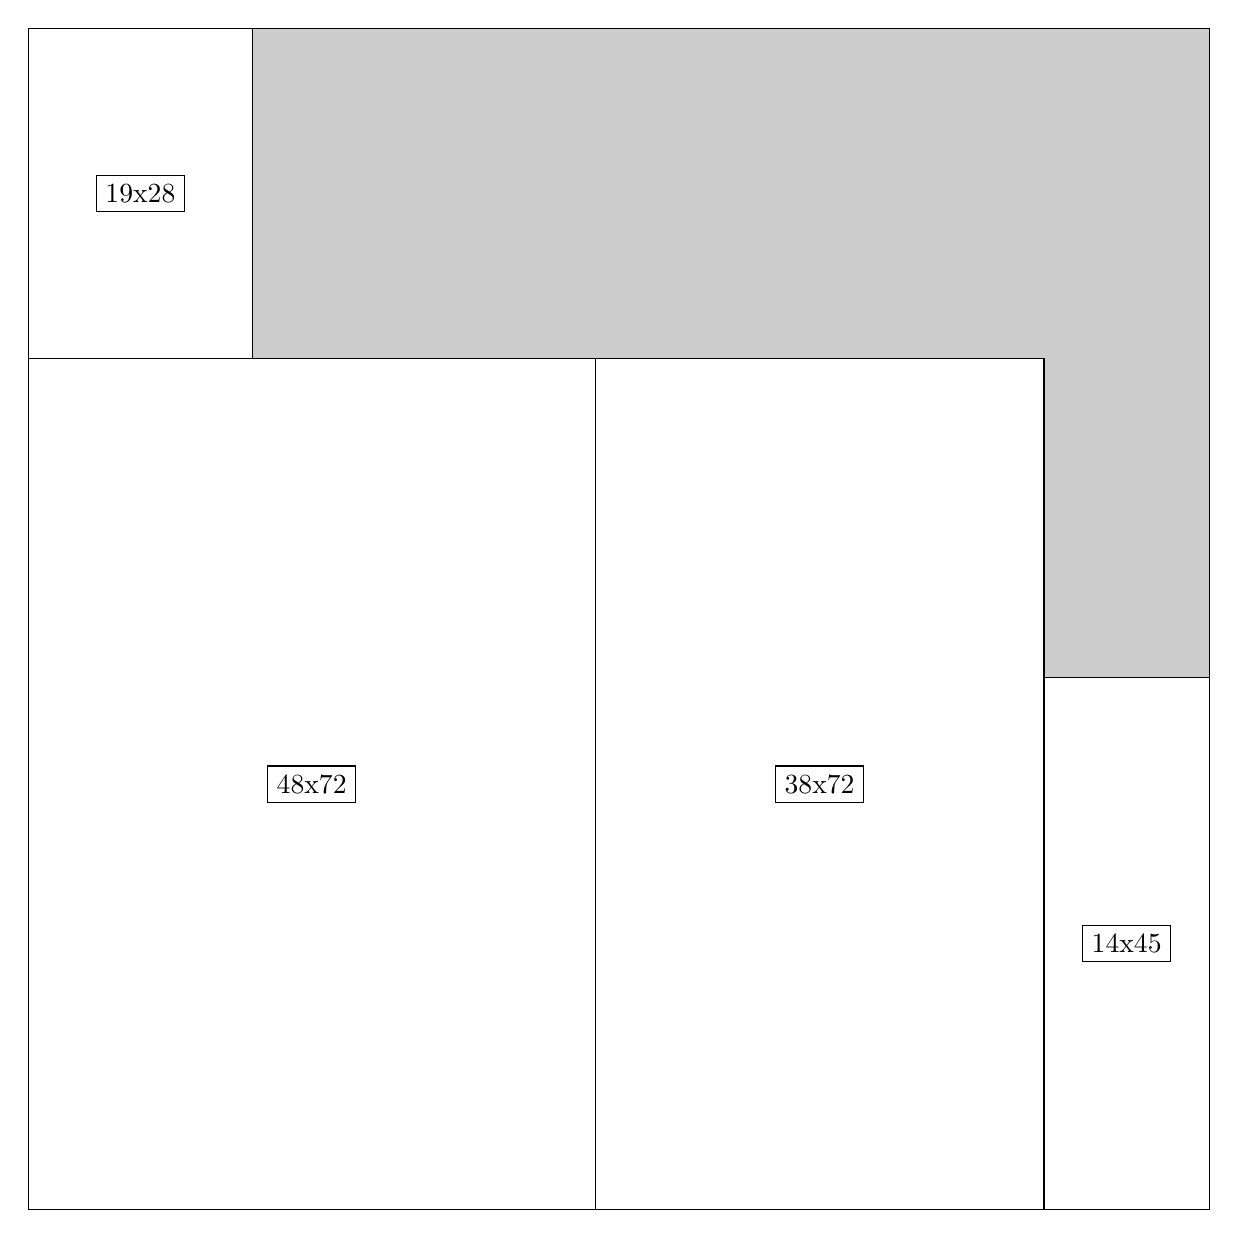
\begin{tikzpicture}[shorten >=1pt,scale=1.0,every node/.style={scale=1.0},->]
\tikzstyle{vertex}=[circle,fill=black!25,minimum size=14pt,inner sep=0pt]
\filldraw[fill=gray!40!white, draw=black] (0,0) rectangle (15.0,15.0);
\foreach \name/\x/\y/\w/\h in {48x72/0.0/0.0/7.199999999999999/10.799999999999999,38x72/7.199999999999999/0.0/5.7/10.799999999999999,14x45/12.9/0.0/2.1/6.75,19x28/0.0/10.799999999999999/2.85/4.2}
\filldraw[fill=white!40!white, draw=black] (\x,\y) rectangle node[draw] (\name) {\name} ++(\w,\h);
\end{tikzpicture}


w =48 , h =72 , x =0 , y =0 , v =3456
\par
w =38 , h =72 , x =48 , y =0 , v =2736
\par
w =14 , h =45 , x =86 , y =0 , v =630
\par
w =19 , h =28 , x =0 , y =72 , v =532
\par
\newpage


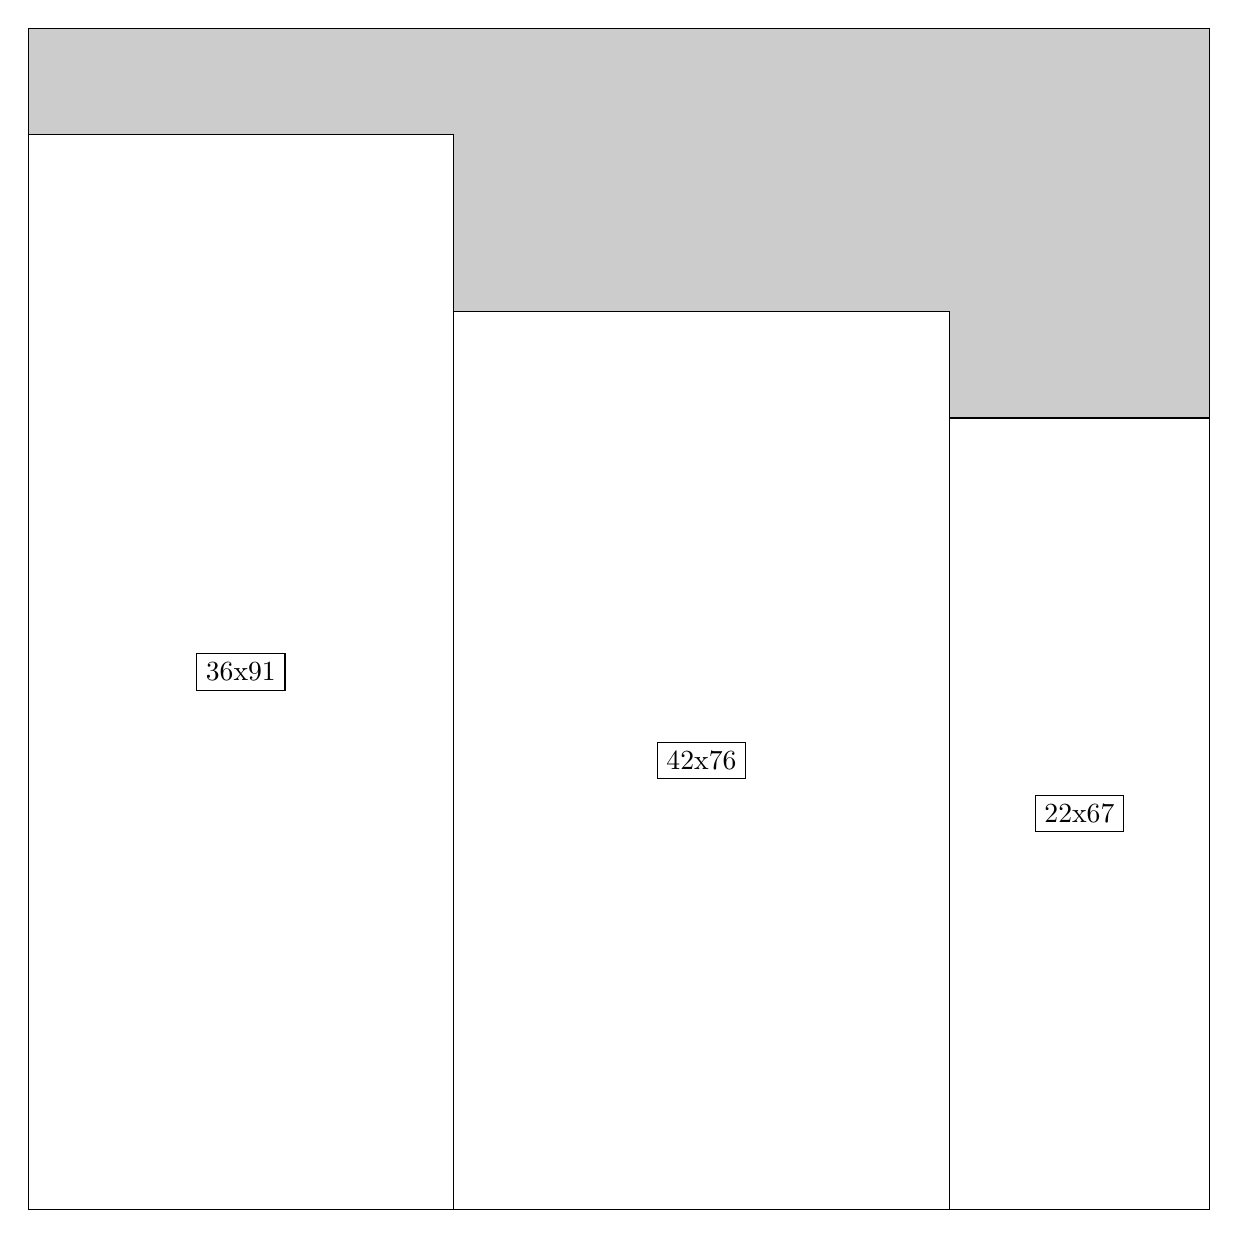
\begin{tikzpicture}[shorten >=1pt,scale=1.0,every node/.style={scale=1.0},->]
\tikzstyle{vertex}=[circle,fill=black!25,minimum size=14pt,inner sep=0pt]
\filldraw[fill=gray!40!white, draw=black] (0,0) rectangle (15.0,15.0);
\foreach \name/\x/\y/\w/\h in {36x91/0.0/0.0/5.3999999999999995/13.65,42x76/5.3999999999999995/0.0/6.3/11.4,22x67/11.7/0.0/3.3/10.049999999999999}
\filldraw[fill=white!40!white, draw=black] (\x,\y) rectangle node[draw] (\name) {\name} ++(\w,\h);
\end{tikzpicture}


w =36 , h =91 , x =0 , y =0 , v =3276
\par
w =42 , h =76 , x =36 , y =0 , v =3192
\par
w =22 , h =67 , x =78 , y =0 , v =1474
\par
\newpage


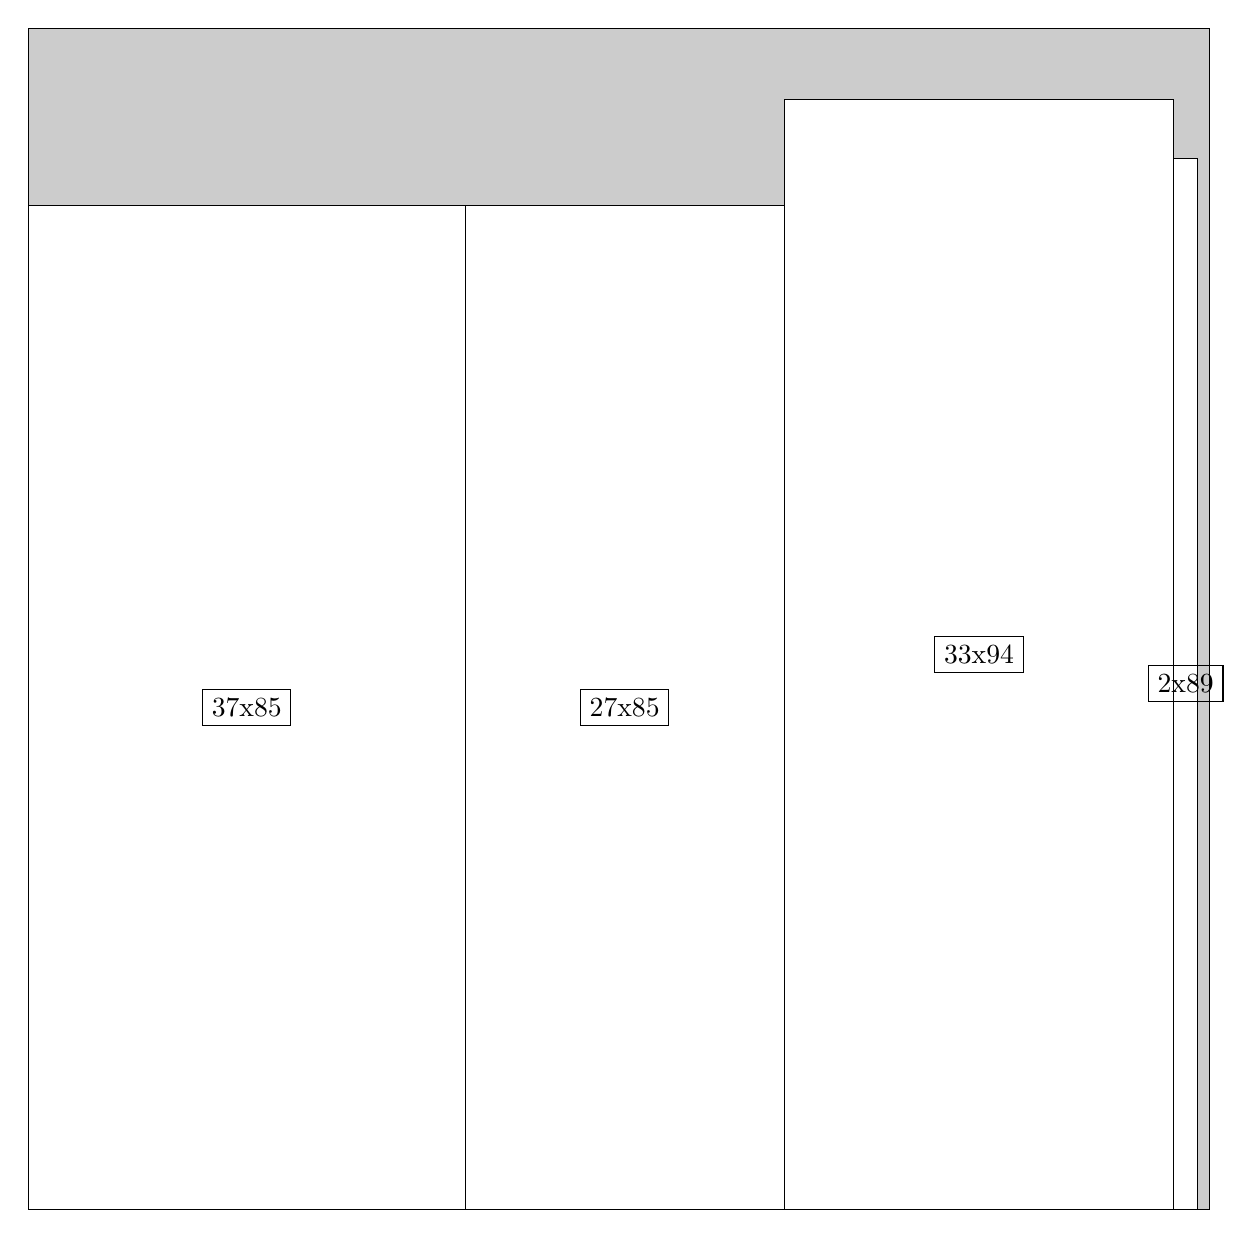
\begin{tikzpicture}[shorten >=1pt,scale=1.0,every node/.style={scale=1.0},->]
\tikzstyle{vertex}=[circle,fill=black!25,minimum size=14pt,inner sep=0pt]
\filldraw[fill=gray!40!white, draw=black] (0,0) rectangle (15.0,15.0);
\foreach \name/\x/\y/\w/\h in {37x85/0.0/0.0/5.55/12.75,33x94/9.6/0.0/4.95/14.1,27x85/5.55/0.0/4.05/12.75,2x89/14.549999999999999/0.0/0.3/13.35}
\filldraw[fill=white!40!white, draw=black] (\x,\y) rectangle node[draw] (\name) {\name} ++(\w,\h);
\end{tikzpicture}


w =37 , h =85 , x =0 , y =0 , v =3145
\par
w =33 , h =94 , x =64 , y =0 , v =3102
\par
w =27 , h =85 , x =37 , y =0 , v =2295
\par
w =2 , h =89 , x =97 , y =0 , v =178
\par
\newpage


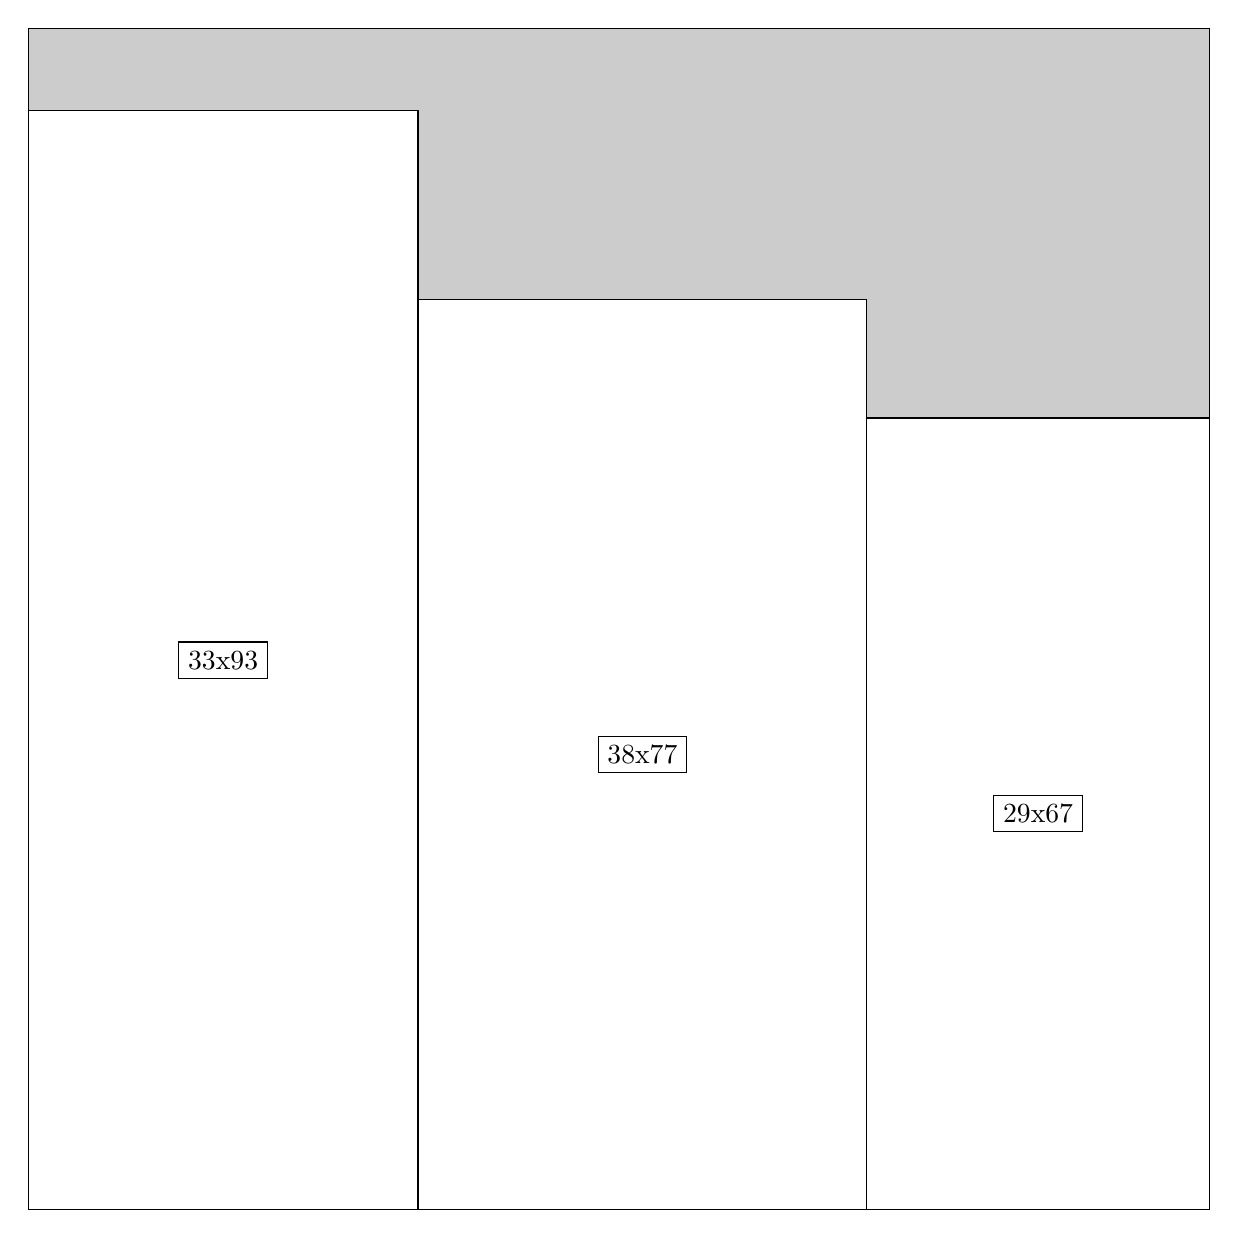
\begin{tikzpicture}[shorten >=1pt,scale=1.0,every node/.style={scale=1.0},->]
\tikzstyle{vertex}=[circle,fill=black!25,minimum size=14pt,inner sep=0pt]
\filldraw[fill=gray!40!white, draw=black] (0,0) rectangle (15.0,15.0);
\foreach \name/\x/\y/\w/\h in {33x93/0.0/0.0/4.95/13.95,38x77/4.95/0.0/5.7/11.549999999999999,29x67/10.65/0.0/4.35/10.049999999999999}
\filldraw[fill=white!40!white, draw=black] (\x,\y) rectangle node[draw] (\name) {\name} ++(\w,\h);
\end{tikzpicture}


w =33 , h =93 , x =0 , y =0 , v =3069
\par
w =38 , h =77 , x =33 , y =0 , v =2926
\par
w =29 , h =67 , x =71 , y =0 , v =1943
\par
\newpage


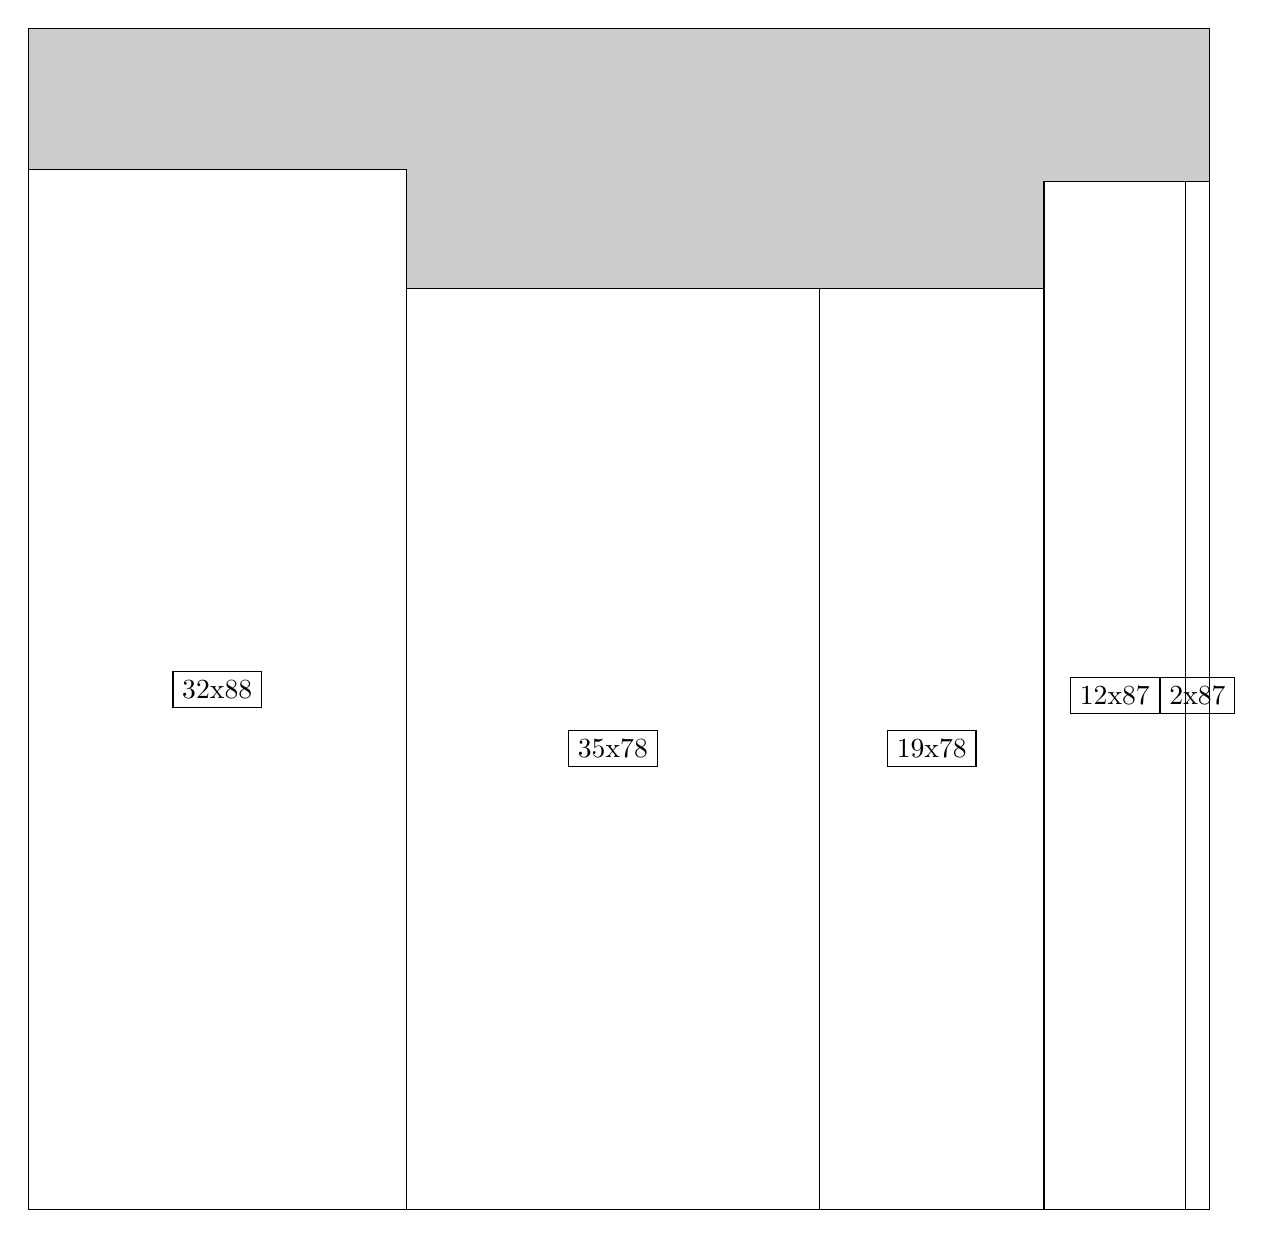
\begin{tikzpicture}[shorten >=1pt,scale=1.0,every node/.style={scale=1.0},->]
\tikzstyle{vertex}=[circle,fill=black!25,minimum size=14pt,inner sep=0pt]
\filldraw[fill=gray!40!white, draw=black] (0,0) rectangle (15.0,15.0);
\foreach \name/\x/\y/\w/\h in {32x88/0.0/0.0/4.8/13.2,35x78/4.8/0.0/5.25/11.7,12x87/12.9/0.0/1.7999999999999998/13.049999999999999,19x78/10.049999999999999/0.0/2.85/11.7,2x87/14.7/0.0/0.3/13.049999999999999}
\filldraw[fill=white!40!white, draw=black] (\x,\y) rectangle node[draw] (\name) {\name} ++(\w,\h);
\end{tikzpicture}


w =32 , h =88 , x =0 , y =0 , v =2816
\par
w =35 , h =78 , x =32 , y =0 , v =2730
\par
w =12 , h =87 , x =86 , y =0 , v =1044
\par
w =19 , h =78 , x =67 , y =0 , v =1482
\par
w =2 , h =87 , x =98 , y =0 , v =174
\par
\newpage


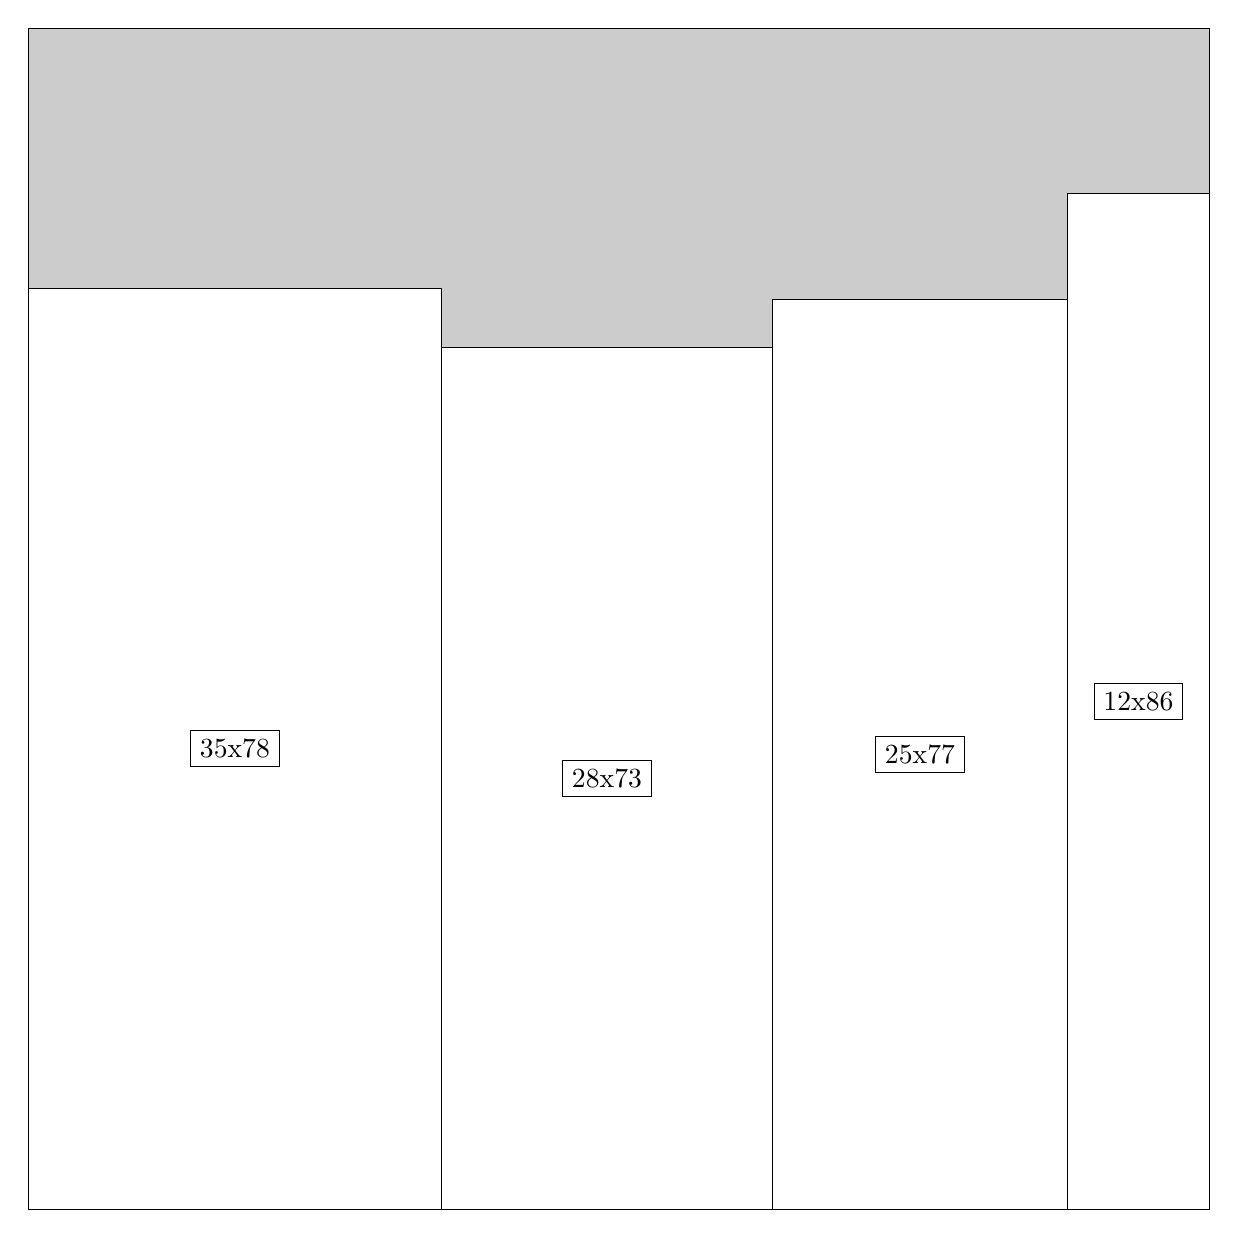
\begin{tikzpicture}[shorten >=1pt,scale=1.0,every node/.style={scale=1.0},->]
\tikzstyle{vertex}=[circle,fill=black!25,minimum size=14pt,inner sep=0pt]
\filldraw[fill=gray!40!white, draw=black] (0,0) rectangle (15.0,15.0);
\foreach \name/\x/\y/\w/\h in {35x78/0.0/0.0/5.25/11.7,28x73/5.25/0.0/4.2/10.95,25x77/9.45/0.0/3.75/11.549999999999999,12x86/13.2/0.0/1.7999999999999998/12.9}
\filldraw[fill=white!40!white, draw=black] (\x,\y) rectangle node[draw] (\name) {\name} ++(\w,\h);
\end{tikzpicture}


w =35 , h =78 , x =0 , y =0 , v =2730
\par
w =28 , h =73 , x =35 , y =0 , v =2044
\par
w =25 , h =77 , x =63 , y =0 , v =1925
\par
w =12 , h =86 , x =88 , y =0 , v =1032
\par
\newpage


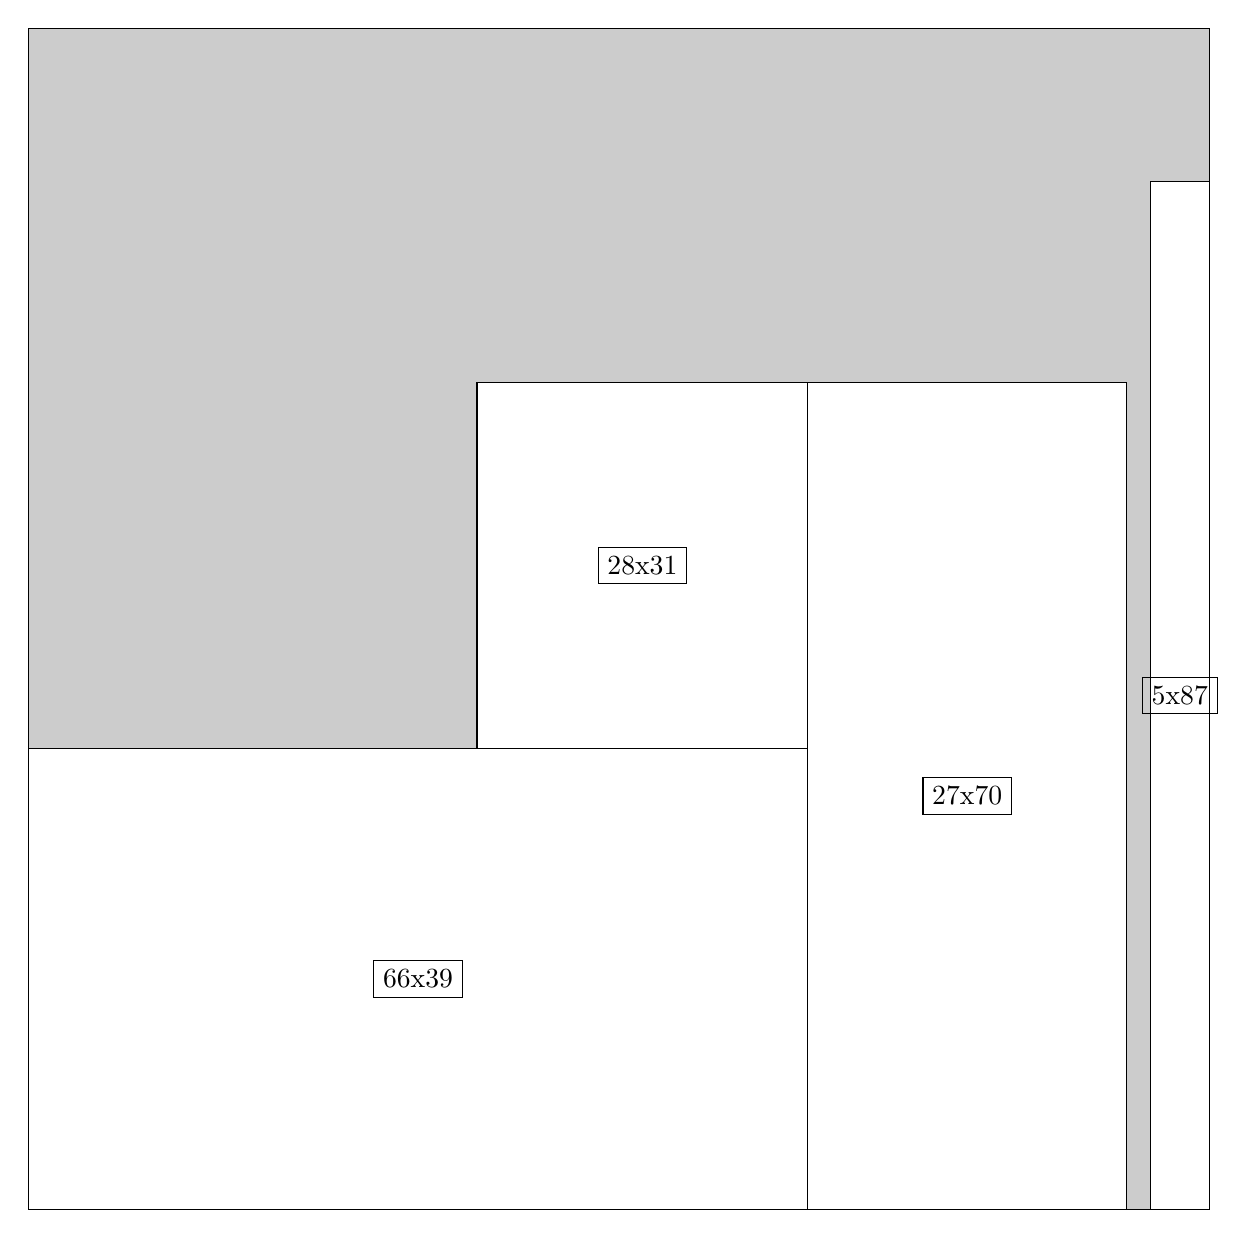
\begin{tikzpicture}[shorten >=1pt,scale=1.0,every node/.style={scale=1.0},->]
\tikzstyle{vertex}=[circle,fill=black!25,minimum size=14pt,inner sep=0pt]
\filldraw[fill=gray!40!white, draw=black] (0,0) rectangle (15.0,15.0);
\foreach \name/\x/\y/\w/\h in {66x39/0.0/0.0/9.9/5.85,27x70/9.9/0.0/4.05/10.5,28x31/5.7/5.85/4.2/4.6499999999999995,5x87/14.25/0.0/0.75/13.049999999999999}
\filldraw[fill=white!40!white, draw=black] (\x,\y) rectangle node[draw] (\name) {\name} ++(\w,\h);
\end{tikzpicture}


w =66 , h =39 , x =0 , y =0 , v =2574
\par
w =27 , h =70 , x =66 , y =0 , v =1890
\par
w =28 , h =31 , x =38 , y =39 , v =868
\par
w =5 , h =87 , x =95 , y =0 , v =435
\par
\newpage


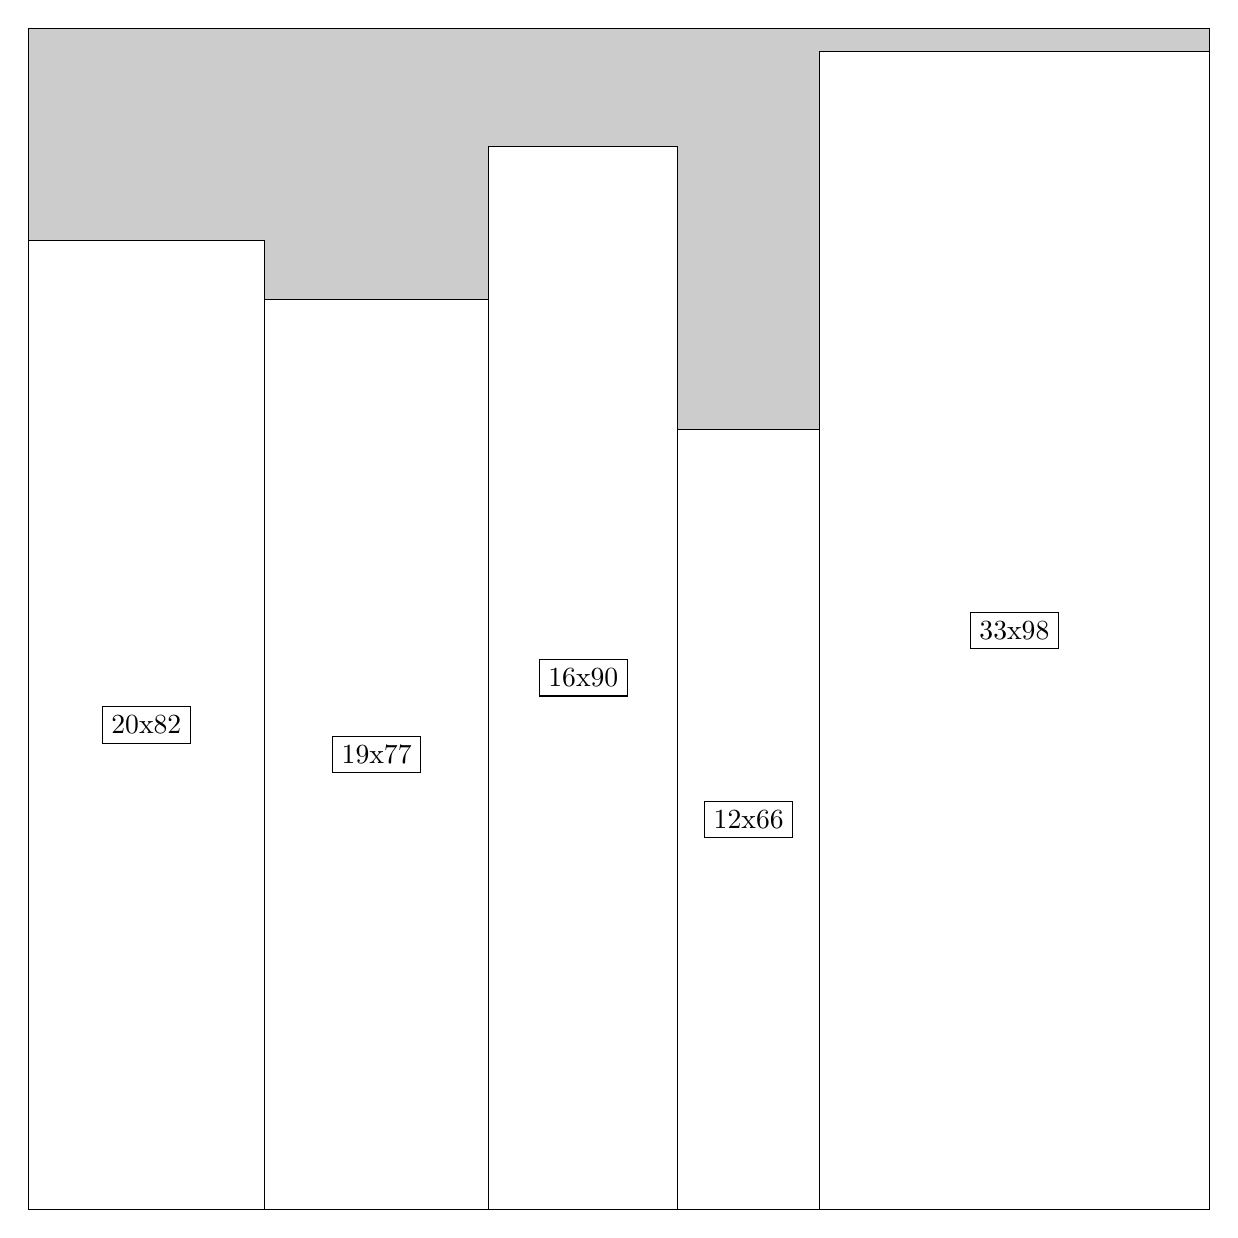
\begin{tikzpicture}[shorten >=1pt,scale=1.0,every node/.style={scale=1.0},->]
\tikzstyle{vertex}=[circle,fill=black!25,minimum size=14pt,inner sep=0pt]
\filldraw[fill=gray!40!white, draw=black] (0,0) rectangle (15.0,15.0);
\foreach \name/\x/\y/\w/\h in {33x98/10.049999999999999/0.0/4.95/14.7,20x82/0.0/0.0/3.0/12.299999999999999,19x77/3.0/0.0/2.85/11.549999999999999,16x90/5.85/0.0/2.4/13.5,12x66/8.25/0.0/1.7999999999999998/9.9}
\filldraw[fill=white!40!white, draw=black] (\x,\y) rectangle node[draw] (\name) {\name} ++(\w,\h);
\end{tikzpicture}


w =33 , h =98 , x =67 , y =0 , v =3234
\par
w =20 , h =82 , x =0 , y =0 , v =1640
\par
w =19 , h =77 , x =20 , y =0 , v =1463
\par
w =16 , h =90 , x =39 , y =0 , v =1440
\par
w =12 , h =66 , x =55 , y =0 , v =792
\par
\newpage


\end{document}